\documentclass{book}
\usepackage{a4wide}

%% possible fonts -- in order of preference
%%\usepackage{palatino}
\usepackage{bookman}
%%\usepackage{charter}
%%\usepackage{newcent}
%%\usepackage{times}
%%\usepackage{avant}
%%\usepackage{helvet}
%%\usepackage{sans}
%%\usepackage{chancery}

\usepackage[T1]{fontenc}
\usepackage{setspace}
\usepackage{ifpdf}
\usepackage{makeidx}
\usepackage{longtable}  %% page wrapping table environment
\usepackage{colortbl}   %% colors for tables
\usepackage{fancyvrb}   %% the "Verbatim" environment
\usepackage{fancyhdr}   %% custom headers and footers
\usepackage{multicol}
\usepackage{listings}   %% source code listings with syntax highlight (lstxxx commands)
\usepackage[tight]{shorttoc}   %% for generating a second table of contents, only containing chapter titles
\usepackage{bytefield}  %% for drawing protocol frames
\usepackage{paralist}   %% for compact lists
\usepackage{tocbibind}  %% makes Bibliography and Index show up in TOC
\settocbibname{References}

\setlength{\textwidth}{160mm}
%\setlength{\oddsidemargin}{12.5mm}
%\setlength{\evensidemargin}{12.5mm}
%\setlength{\topmargin}{0mm}
\setlength{\textheight}{220mm}
%\setlength{\parskip}{1ex}
%\setlength{\parindent}{5ex}

\renewcommand{\bottomfraction}{0.9}
\renewcommand{\topfraction}{0.9}
\renewcommand{\floatpagefraction}{0.9}

%% try to cure overfull hboxes
%% \tolerance=500

%% for navigation in dvi files, only needed by old teTeX versions
%%\usepackage{srcltx}


%% try this for spell checking: cat ess2002.tex | ispell -l -t -a | sort | uniq | more

%%
%% OMNeT++ logo, use as {\opp}
%%
\makeatletter
%%\DeclareRobustCommand{\omnetpp}{OM\-NeT\kern-.18em++\@}
\DeclareRobustCommand{\omnetpp}{OMNeT++\@}
\makeatother

\newcommand{\opp}{\omnetpp}

%%
%% PDF Header
%%
% note: \ifpdf now comes from the ifpdf package
%\newif\ifpdf
%\ifx\pdfoutput\undefined
%  \pdffalse
%\else
%  \pdfoutput=1
%  \pdftrue
%\fi
%% PDF-Info
\ifpdf
  \usepackage[pdftex]{graphicx}
  \usepackage[plainpages=false,linktocpage,bookmarksnumbered=true,pdftex]{hyperref}   %% automatic hyperlinking
  \pdfcompresslevel=9
  \pdfinfo{/Author (Andras Varga and others)
    /Title (INET Framework Manual)
    /Subject ()
    /Keywords (INET, INETMANET, OMNeT++, manual)}
\else
  \usepackage{graphicx}
  \usepackage[plainpages=false]{hyperref}   %% automatic hyperlinking
\fi

%%
%% Generate Index
%%
\makeindex


%%
%% Link colors (hyperref package)
%%
\definecolor{MyDarkBlue}{rgb}{0.16,0.16,0.5}
%% XXX the next line apparently screws up all links except in TOC! they'll be colored nicely, but won't work.
%\hypersetup{
%    colorlinks=true,
%    linkcolor=MyDarkBlue,
%    anchorcolor=MyDarkBlue,
%    citecolor=MyDarkBlue,
%    filecolor=MyDarkBlue,
%    menucolor=MyDarkBlue,
%    runcolor=MyDarkBlue,
%    urlcolor=blue,
%}

%%
%% Heading and Footer
%%
\pagestyle{fancy}
\fancyhf{}
\renewcommand{\footrulewidth}{0.5pt}
\renewcommand{\chaptermark}[1]{\markboth{#1}{}}
\lhead{{\opp} Manual -- \leftmark}
\rfoot{\thepage}

%% this is used for chapter start pages
\fancypagestyle{plain}{
    \rfoot{\thepage}
}

%%
%% Use \begin{graybox}...\end{graybox} for notes
%%
\definecolor{MyGray}{rgb}{0.85,0.85,1.0}
\makeatletter\newenvironment{graybox}%
   {\begin{flushright}\begin{lrbox}{\@tempboxa}\begin{minipage}[r]{0.95\textwidth}}%
   {\end{minipage}\end{lrbox}\colorbox{MyGray}{\usebox{\@tempboxa}}\end{flushright}}%
\makeatother


\newenvironment{note}{\begin{graybox}\textbf{NOTE: }}{\end{graybox}}
\newenvironment{warning}{\begin{graybox}\textbf{WARNING: }}{\end{graybox}}
\newenvironment{caution}{\begin{graybox}\textbf{CAUTION: }}{\end{graybox}}
\newenvironment{rationale}{\begin{graybox}\textbf{Rationale: }}{\end{graybox}}
\newenvironment{important}{\begin{graybox}\textbf{IMPORTANT: }}{\end{graybox}}

%%
%% Set up listings package
%%
\lstloadlanguages{C++,make,perl,tcl,XML,R,Matlab}

%% See listings.pdf,pp20
\lstdefinelanguage{NED} {
    morekeywords={allowunconnected,bool,channel,channelinterface,connections,const,
                  default,double,extends,false,for,gates,if,import,index,inout,input,
                  int,like,module,moduleinterface,network,output,package,parameters,
                  property,simple,sizeof,string,submodules,this,true,types,volatile,
                  xml,xmldoc},
    sensitive=true,
    morecomment=[l]{//},
    morestring=[b]",
}
\lstdefinelanguage{MSG} {
    morekeywords={abstract,bool,char,class,cplusplus,double,enum,extends,false,
                  fields,int,long,message,namespace,noncobject,packet,properties,
                  readonly,short,string,struct,true,unsigned},
    sensitive=true,
    morecomment=[l]{//},
    morestring=[b]",
}
\lstdefinelanguage{inifile} {
    morekeywords={},
    sensitive=true,
    morecomment=[l]{\#},
    morestring=[b]",
}
\lstdefinelanguage{pseudocode} {
    morekeywords={if,then,else,otherwise,whenever,while},
    sensitive=true,
    morecomment=[l]{//},
    morestring=[b]",
    mathescape=true,
}

%% thick ruler on the left; also, designate backtick as LaTeX escape character
%% (e.g. \opp needs to be written as `\opp` inside listing blocks)
\lstset{
    escapechar=`,
    basicstyle=\ttfamily,
    showstringspaces=false,
    frame=leftline,
    framesep=10pt,
    framerule=3pt,
    xleftmargin=15pt
}

\definecolor{NEDRulerColor}{rgb}{0.8,1.0,0.8}  % pale green
\definecolor{MSGRulerColor}{rgb}{0.8,1.0,0.8}  % pale green
\definecolor{CPPRulerColor}{rgb}{0.8,0.8,1.0}  % pale blue
\definecolor{IniRulerColor}{rgb}{0.9,0.9,0.2}  % pale yellow
\definecolor{FileListingRulerColor}{rgb}{0.85,0.85,0.85}  % grey
%\definecolor{CommandLineRulerColor}{rgb}{0.9,0.9,0.2}
\definecolor{PseudoCodeRulerColor}{rgb}{0.0,1.0,1.0}  % cyan

%% See listings.pdf,pp39
\lstnewenvironment{ned}
    {\lstset{language=NED,rulecolor=\color{NEDRulerColor}}}
    {}
\lstnewenvironment{msg}
    {\lstset{language=MSG,rulecolor=\color{MSGRulerColor}}}
    {}
\lstnewenvironment{cpp}
    {\lstset{language=C++,rulecolor=\color{CPPRulerColor}}}
    {}
\lstnewenvironment{inifile}
    {\lstset{language=inifile,rulecolor=\color{IniRulerColor}}}
    {}
\lstnewenvironment{filelisting}
    {\lstset{language={},rulecolor=\color{FileListingRulerColor}}}
    {}
\lstnewenvironment{commandline}
    {\lstset{language={},framesep=11pt,framerule=1pt,xleftmargin=16pt}}
    {}
\lstnewenvironment{pseudocode}
    {\lstset{language=pseudocode,rulecolor=\color{PseudoCodeRulerColor}}}
    {}

%%
%% some customization
%%
\setlength{\parindent}{0pt}
\setlength{\parskip}{1ex}

%%
%% Shortcuts
%%
\newcommand{\appendixchapter}{\chapter} %% html converter needs to know which chapters are appendices

\newcommand{\tbf}{\textbf} %% bold faced text
\newcommand{\ttt}{\texttt} %% type writer font text

\newcommand{\tab}{\hspace*{5mm}} %% tabulator settings

\newcommand{\new}{$^{New!}$}
\newcommand{\changed}{$^{Changed!}$}

%% Colordefinition for table header rows (requires package colortbl)
\newcommand{\tabheadcol}{\rowcolor[gray]{0.8}}

%%
%% Module parameters list
%%
\newenvironment{params}{\begin{itemize}}{\end{itemize}}
\newcommand{\param}[2]{\item \fpar{#1}: #2}

%%
%% Function/Class/Macro/Variable/Program/Parameter/Define names
%%
%% Write the names in type writer font and do an index entry
%% Allows word wrap by automatic hyphenation
%%
%% Usage: \ffunc{take()}
%%    or: \ffunc[take()]{take(obj)}
%% the second form uses the bracketed word for the index entry
%%

%% NED type names
\newcommand{\nedtype}[2][\DefaultOpt]{\def\DefaultOpt{#2}%
  \index{#1}%
  \texttt{\hyphenchar\font=`\-\relax#2}}

%% MSG type names
\newcommand{\msgtype}[2][\DefaultOpt]{\def\DefaultOpt{#2}%
  \index{#1}%
  \texttt{\hyphenchar\font=`\-\relax#2}}

%% Function names
\newcommand{\ffunc}[2][\DefaultOpt]{\def\DefaultOpt{#2}%
  \index{#1}%
  \texttt{\hyphenchar\font=`\-\relax#2}}

%% Class names
\newcommand{\cppclass}[2][\DefaultOpt]{\def\DefaultOpt{#2}%
  \index{#1}%
  \texttt{\hyphenchar\font=`\-\relax#2}}

%% Macro names
\newcommand{\fmac}[2][\DefaultOpt]{\def\DefaultOpt{#2}%
  \index{#1}%
  \texttt{\hyphenchar\font=`\-\relax#2}}

%% Variable names
\newcommand{\fvar}[2][\DefaultOpt]{\def\DefaultOpt{#2}%
  \index{#1}%
  \texttt{\hyphenchar\font=`\-\relax#2}}

%% Program names
\newcommand{\fprog}[2][\DefaultOpt]{\def\DefaultOpt{#2}%
  \index{#1}%
  \texttt{\hyphenchar\font=`\-\relax#2}}

%% Parameter names
\newcommand{\fpar}[2][\DefaultOpt]{\def\DefaultOpt{#2}%
  \index{#1}%
  \texttt{\hyphenchar\font=`\-\relax#2}}

%% Defines
\newcommand{\fdef}[2][\DefaultOpt]{\def\DefaultOpt{#2}%
  \index{#1}%
  \texttt{\hyphenchar\font=`\-\relax#2}}

%% NED/MSG properties
\newcommand{\fprop}[2][\DefaultOpt]{\def\DefaultOpt{#2}%
  \index{#1}%
  \texttt{\hyphenchar\font=`\-\relax#2}}

%% Keywords (NED, MSG)
\newcommand{\fkeyword}[2][\DefaultOpt]{\def\DefaultOpt{#2}%
  \index{#1}%
  \textbf{\texttt{\hyphenchar\font=`\-\relax#2}}}

%% Configuration options
\newcommand{\fconfig}[2][\DefaultOpt]{\def\DefaultOpt{#2}%
  \index{#1}%
  \textbf{\texttt{\hyphenchar\font=`\-\relax#2}}}

%% File names
\newcommand{\ffilename}[2][\DefaultOpt]{\def\DefaultOpt{#2}%
  \index{#1}%
  \texttt{\hyphenchar\font=`\-\relax#2}}

%% Signals
\newcommand{\fsignal}[2][\DefaultOpt]{\def\DefaultOpt{#2}%
  \index{#1}%
  \texttt{\hyphenchar\font=`\-\relax#2}}

\newcommand{\fgate}[1]{\texttt{\hyphenchar\font=`\-\relax#1}}

%% do not number subsubsections
%\setcounter{secnumdepth}{4}

% limit the depth of TOC
\setcounter{tocdepth}{2}

%%
%% Start of document
%%
\begin{document}

%% set the image type preference
\DeclareGraphicsExtensions{.pdf,.png}

\pagestyle{empty}
\pagenumbering{roman}

%% %%\begin{figure}[htbp]
%%\begin{center}
%%\includegraphics[width=3.648in, height=0.990in]{figures/usmanFig1}
%%\end{center}
%% %%\end{figure}

%% the following {center} is a trick -- vspace does nothing if there's
%% nothing above it in the page
\begin{center}\end{center}
\vspace{16em}
\hrule
\vspace{2em}
\begin{center}
{\LARGE INET Framework for OMNeT++}\\
\vspace{1em}
{\large Manual}\\
\end{center}
\vspace{2em}
\hrule

%\vspace{4em}
%by {\large Andr\'{a}s Varga}
%\vspace{3em}

\vspace{8em}

\begin{center}
% \textit{WORK IN PROGRESS}
\textit{Generated on \today}
\end{center}



%%% Local Variables:
%%% mode: latex
%%% TeX-master: "usman"
%%% End:

\cleardoublepage

%%\setcounter{page}{1}
%\newpage
%%\pagenumbering{roman}

%% \shorttableofcontents{Chapters}{0}
%% \cleardoublepage

\tableofcontents
\cleardoublepage

\pagestyle{fancy}
\pagenumbering{arabic}

\chapter{Introduction}
\label{cha:introduction}


\section{What is INET Framework}

INET Framework is an open-source model library for the OMNeT++ simulation
environment. It provides protocols, agents and other models for researchers 
and students working with communication networks. INET is especially useful 
when designing and validating new protocols, or exploring new or exotic scenarios.

INET supports a wide class of communication networks, including wired, 
wireless, mobile, ad hoc and sensor networks.  It contains models for 
the Internet stack (TCP, UDP, IPv4, IPv6, OSPF, BGP, etc.), link layer protocols 
(Ethernet, PPP, IEEE 802.11, various sensor MAC protocols, etc), 
refined support for the wireless physical layer, MANET routing protocols, 
DiffServ, MPLS with LDP and RSVP-TE signalling, several application models,
and many other protocols and components. It also provides support for 
node mobility, advanced visualization, network emulation and more. 

Several other simulation frameworks take INET as a base, and extend it 
into specific directions, such as vehicular networks, overlay/peer-to-peer 
networks, or LTE.

\section{Designed for Experimentation}

INET is built around the concept of modules that communicate by message passing.
Agents and network protocols are represented by components, which can be freely
combined to form hosts, routers, switches, and other networking devices. 
New components can be programmed by the user, and existing components have 
been written so that they are easy to understand and modify.

INET benefits from the infrastructure provided by OMNeT++. Beyond making 
use of the services provided by the OMNeT++ simulation kernel and library
(component model, parameterization, result recording, etc.), this also means
that models may be developed, assembled, parameterized, run, and their 
results evaluted from the comfort of the OMNeT++ Simulation IDE, or 
from the command line.

INET Framework is maintained by the OMNeT++ team for the community, 
utilizing patches and new models contributed by members of the community.

\section{Scope of this Manual}

This manual is written for users who are interested in assembling
simulations using the components provided by the INET Framework.
(In contrast, if you are interested in modifing INET's components or plan 
to extend INET with new protocols or other components using C++, 
we recommend the \textit{INET Developers Guide}.)

This manual does not attempt to be a reference for INET. It concentrates
on conveying the big picture, and does not attempt to cover all 
components, or try to document the parameters, gates, statistics or 
precise operation of individual components. For such information, 
users should refer to the \textit{INET Reference}, a web-based 
cross-referenced documentation generated from NED and MSG files.
 
A working knowledge of OMNeT++ is assumed.


%%% Local Variables:
%%% mode: latex
%%% TeX-master: "usman"
%%% End:


\cleardoublepage

\chapter{Using the INET Framework}
\label{cha:usage}

\section{Installation}
\label{sec:usage:installation}

There are several ways to install the INET Framework:

\begin{itemize}
  \item Let the OMNeT++ IDE download and install it for you.
      This is the easiest way. Just accept the offer to install INET
      in the dialog that comes up when you first start the IDE, or
      choose \textit{Help > Install Simulation Models} any time later.
  \item From INET Framework web site, \textit{http://inet.omnetpp.org}.
      The IDE always installs the last stable version compatible with
      your version of OMNeT++. If you need some other version, they
      are available for download from the web site. Installation
      instructions are also provided there.
  \item From GitHub. If you have experience with \textit{git},
      clone the INET Framework project (\ttt{inet\--frame\-work/inet}),
      check out the revision of your choice, and follow the INSTALL
      file in the project root.
\end{itemize}


\section{Installing INET Extensions}
\label{sec:usage:installing-inet-extensions}

If you plan to make use of INET extensions (e.g. Veins or SimuLTE),
follow the installation instructions provided with them.

In the absence of specific instructions, the following procedure usually works:

\begin{itemize}
 \item First, check if the project root contains a file named \ttt{.project}.
 \item If it does, then the project can be imported into the IDE (use \textit{File > Import >
    General > Existing Project} into workspace). make sure that the project is recognized
    as an OMNeT++ project (the \textit{Project Properties} dialog contains a page
    titled \textit{OMNeT++}), and it lists the INET project as dependency
    (check the \textit{Project References} page in the \textit{Project Properties} dialog).
 \item If there is no \ttt{.project} file, you can create an empty OMNeT++
    project using the \textit{New OMNeT++ Project} wizard in \textit{File > New},
    add the INET project as dependency using the \textit{Project References} page
    in the \textit{Project Properties} dialog, and copy the source files into the project.
\end{itemize}

\section{Getting Familiar with INET}
\label{sec:usage:getting-familiar-with-inet}

The INET Framework builds upon OMNeT++, and uses the same concept: modules
that communicate by message passing. Hosts, routers, switches and other
network devices are represented by OMNeT++ compound modules. These compound
modules are assembled from simple modules that represent protocols,
applications, and other functional units. A network is again an OMNeT++
compound module that contains host, router and other modules.

Modules are organized into a directory structure that roughly follows
OSI layers:

\begin{itemize}
  \item \ttt{src/inet/applications/} -- traffic generators and application models
  \item \ttt{src/inet/transportlayer/} -- transport layer protocols
  \item \ttt{src/inet/networklayer/} -- network layer protocols and accessories
  \item \ttt{src/inet/linklayer/} -- link layer protocols and accessories
  \item \ttt{src/inet/physicallayer/} -- physical layer models
  \item \ttt{src/inet/routing/} -- routing protocols (internet and ad hoc)
  \item \ttt{src/inet/mobility/} -- mobility models
  \item \ttt{src/inet/power/} -- energy consumption modeling
  \item \ttt{src/inet/environment/} -- model of the physical environment
  \item \ttt{src/inet/node/} -- preassembled network node models
  \item \ttt{src/inet/visualizer/} -- visualization components (2D and 3D)
  \item \ttt{src/inet/common/} -- miscellaneous utility components
\end{itemize}

The OMNeT++ NED language uses hierarchical packages names. Packages correspond
to directories under \ttt{src/}, so e.g. the \ttt{src/inet/transportlayer/tcp}
directory corresponds to the \ttt{inet.transportlayer.tcp} NED package.

For modularity, the INET Framework has about 80 \textit{project features}
(parts of the codebase that can be disabled as a unit) defined. Not all project
features are enabled in the default setup after installation. You can review
the list of available project features in the \textit{Project | Project Features...}
dialog in the IDE. If you want to know more about project features, refer to the
\textit{OMNeT++ User Guide}.


%%% Local Variables:
%%% mode: latex
%%% TeX-master: "usman"
%%% End:


\cleardoublepage

\chapter{Node Architecture}
\label{cha:node-architecture}

\section{Addresses}

The INET Framework uses a number of C++ classes to represent various
addresses in the network. These classes support initialization and
assignment from binary and string representation of the address, and
accessing the address in both forms. (Storage is in binary form). They also
support the "unspecified" special value (and the \ffunc{isUnspecified()}
method) that corresponds to the all-zeros address.

\begin{itemize}
  \item \cppclass{MacAddress} represents a 48-bit IEEE 802 MAC address. The
    textual notation it understands and produces is hex string.

  \item \cppclass{Ipv4Address} represents a 32-bit IPv4 address. It can parse
    and produce textual representations in the "dotted decimal" syntax.

  \item \cppclass{Ipv6Address} represents a 128-bit IPv6 address. It can parse
    and produce address strings in the canonical (RFC 3513) syntax.

  \item \cppclass{L3Address} is conceptually a union of a \cppclass{Ipv4Address}
    and \cppclass{Ipv6Address}: an instance stores either an IPv4 address or an
    IPv6 address. \cppclass{L3Address} is mainly used in the transport layer and above
    to abstract away network addresses. It can be assigned from both \cppclass{Ipv4Address}
    and \cppclass{Ipv6Address}, and can also parse string representations of both.
    The \ffunc{getType()}, \ffunc{toIPv4()} and \ffunc{toIPv6()} methods can be used
    to access the value.
\end{itemize}

\ifdraft TODO
TODO: Resolving addresses with L3AddressResolver
\fi

\section{The Interface Table}

The \nedtype{InterfaceTable} module holds one of the key data structures in
the INET Framework: information about the network interfaces in the host.
The interface table module does not send or receive messages; other modules
access it using standard C++ member function calls.

\ifdraft TODO
\subsection{Accessing the Interface Table}

If a module wants to work with the interface table, first it needs to obtain a
pointer to it. This can be done with the help of the
\cppclass{InterfaceTableAccess} utility class:

\begin{cpp}
IInterfaceTable *ift = InterfaceTableAccess().get();
\end{cpp}

\cppclass{InterfaceTableAccess} requires the interface table module to be a
direct child of the host and be called \ttt{"interfaceTable"} in order to
be able to find it. The \ffunc{get()} method never returns \ttt{NULL}: if
it cannot find the interface table module or cannot cast it to the
appropriate C++ type (\cppclass{IInterfaceTable}), it throws an exception
and stop the simulation with an error message.

For completeness, \cppclass{InterfaceTableAccess} also has a
\ffunc{getIfExists()} method which can be used if the code does not require
the presence of the interface table. This method returns \ttt{NULL} if the
interface table cannot be found.

Note that the returned C++ type is \cppclass{IInterfaceTable}; the initial
"\ttt{I}" stands for "interface". \cppclass{IInterfaceTable} is an abstract
class interface that \cppclass{InterfaceTable} implements. Using the abstract
class interface allows one to transparently replace the interface table with
another implementation, without the need for any change or even
recompilation of the INET Framework.
\fi

\subsection{Interface Entries}

Interfaces in the interface table are represented with the
\cppclass{InterfaceEntry} class. \cppclass{IInterfaceTable} provides member
functions for adding, removing, enumerating and looking up interfaces.

Interfaces have unique names and interface IDs; either can be used to look up
an interface (IDs are naturally more efficient). Interface IDs are invariant to
the addition and removal of other interfaces.

Data stored by an interface entry include:

\begin{itemize}
  \item \textit{name} and \textit{interface ID} (as described above)
  \item \textit{MTU}: Maximum Transmission Unit, e.g. 1500 on Ethernet
  \item several flags:
    \begin{itemize}
      \item \textit{down}: current state (up or down)
      \item \textit{broadcast}: whether the interface supports broadcast
      \item \textit{multicast} whether the interface supports multicast
      \item \textit{pointToPoint}: whether the interface is point-to-point link
      \item \textit{loopback}: whether the interface is a loopback interface
    \end{itemize}
  \item \textit{datarate} in bit/s
  \item \textit{link-layer address} (for now, only IEEE 802 MAC addresses are supported)
  \item \textit{network-layer gate index}: which gate of the network layer within the host the NIC is connected to
  \item \textit{host gate IDs}: the IDs of the input and output gate of the host the NIC is connected to
\end{itemize}

\tbf{Extensibility}. You have probably noticed that the above list does not
contain data such as the IPv4 or IPv6 address of the interface. Such
information is not part of \cppclass{InterfaceEntry} because we do not want
\nedtype{InterfaceTable} to depend on either the IPv4 or the IPv6 protocol
implementation; we want both to be optional, and we want
\nedtype{InterfaceTable} to be able to support possibly other network
protocols as well.

Thus, extra data items are added to \cppclass{InterfaceEntry} via
extension. Two kinds of extensions are envisioned: extension by the link
layer (i.e. the NIC), and extension by the network layer protocol:

\begin{itemize}

\item \tbf{NICs} can extend interface entries via C++ class inheritance, that is, by
simply subclassing \cppclass{InterfaceEntry} and adding extra data and
functions. This is possible because NICs create and register entries in
\nedtype{InterfaceTable}, so in their code one can just write
\ttt{new MyExtendedInterfaceEntry()} instead of \ttt{new InterfaceEntry()}.

\item \textbf{Network layer protocols} cannot add data via subclassing, so
composition has to be used. \cppclass{InterfaceEntry} contains pointers to
network-layer specific data structures. For example, there are pointers to
IPv4 specific data, and IPv6 specific data. These objects can be accessed with
the following \cppclass{InterfaceEntry} member functions: \ffunc{ipv4Data()},
\ffunc{ipv6Data()}, and \ffunc{getGenericNetworkProtocolData()}.
They return pointers of the types \cppclass{Ipv4InterfaceData},
\cppclass{Ipv6InterfaceData}, and \cppclass{GenericNetworkProtocolInterfaceData},
respectively. For illustration, \cppclass{Ipv4InterfaceData} is installed
onto the interface entries by the \nedtype{Ipv4RoutingTable} module, and it
contains data such as the IP address of the interface, the netmask, link
metric for routing, and IP multicast addresses associated with the
interface. A protocol data pointer will be \ttt{NULL} if the corresponding
network protocol is not used in the simulation; for example, in IPv4
simulations only \ffunc{ipv4Data()} will return a non-\ttt{NULL} value.


\end{itemize}


\subsection{Interface Registration}

Interfaces are registered dynamically in the initialization phase by modules
that represent network interface cards (NICs). The INET Framework makes use
of the multi-stage initialization feature of OMNeT++, and interface registration takes
place in the first stage (i.e. stage \ttt{INITSTAGE\_LINK\_LAYER}).

Example code that performs interface registration:

\begin{cpp}
void PPP::initialize(int stage)
{
    if (stage == INITSTAGE_LINK_LAYER) {
        ...
        interfaceEntry = registerInterface(datarate);
    ...
}

InterfaceEntry *PPP::registerInterface(double datarate)
{
    InterfaceEntry *e = new InterfaceEntry(this);

    // interface name: NIC module's name without special characters ([])
    e->setName(OPP_Global::stripnonalnum(getParentModule()->getFullName()).c_str());

    // data rate
    e->setDatarate(datarate);

    // generate a link-layer address to be used as interface token for IPv6
    InterfaceToken token(0, simulation.getUniqueNumber(), 64);
    e->setInterfaceToken(token);

    // set MTU from module parameter of similar name
    e->setMtu(par("mtu"));

    // capabilities
    e->setMulticast(true);
    e->setPointToPoint(true);

    // add
    IInterfaceTable *ift = findModuleFromPar<IInterfaceTable>(par("interfaceTableModule"), this);
    ift->addInterface(e);

    return e;
}
\end{cpp}

\ifdraft TODO
\subsection{Interface Change Notifications}

\nedtype{InterfaceTable} has a change notification mechanism built in, with
the granularity of interface entries.

Clients that wish to be notified when something changes in
\nedtype{InterfaceTable} can subscribe to the following notification
categories in the host's \nedtype{NotificationBoard}:

\begin{itemize}
  \item \tbf{\ttt{NF\_INTERFACE\_CREATED}}: an interface entry has been
    created and added to the interface table
  \item \tbf{\ttt{NF\_INTERFACE\_DELETED}}: an interface entry is going
    to be removed from the interface table. This is a pre-delete
    notification so that clients have access to interface data that are
    possibly needed to react to the change
% TODO hmmm -- rename the constant? also fire a post-change notification??
  \item \tbf{\ttt{NF\_INTERFACE\_CONFIG\_CHANGED}}: a configuration setting
    in an interface entry has changed (e.g. MTU or IP address)
  \item \tbf{\ttt{NF\_INTERFACE\_STATE\_CHANGED}}: a state variable in an
    interface entry has changed (e.g. the up/down flag)
\end{itemize}

In all those notifications, the data field is a pointer to the
corresponding \cppclass{InterfaceEntry} object. This is even true for
\ttt{NF\_INTERFACE\_DELETED} (which is actually a pre-delete notification).
\fi


\section{Communication between protocol layers}

In the INET Framework, when an upper-layer protocol wants to send a data
packet over a lower-layer protocol, the upper-layer module just sends the
message object representing the packet to the lower-layer module, which
will in turn encapsulate it and send it. The reverse process takes place
when a lower layer protocol receives a packet and sends it up after
decapsulation.

It is often necessary to convey extra information with the packet. For
example, when an application-layer module wants to send data over TCP, some
connection identifier needs to be specified for TCP. When TCP sends a
segment over IP, IP will need a destination address and possibly other
parameters like TTL. When IP sends a datagram to an Ethernet interface for
transmission, a destination MAC address must be specified. This extra
information is attached to the message object to as \textit{control info}.

Control info are small value objects, which are attached to packets
(message objects) with its \ttt{setControlInfo()} member function.
Control info only holds auxiliary information for the next protocol layer,
and is not supposed to be sent over the network to other hosts and routers.


\section{NED Conventions}

\subsection{The @node Property}

By convention, compound modules that implement network devices (hosts,
routers, switches, access points, base stations, etc.) are marked with the
\ttt{@node} NED property. As node models may themselves be hierarchical, the
\ttt{@node} property is used by protocol implementations and other simple
modules to determine which ancestor compound module represents the physical
network node they live in.

\subsection{The @labels Module Property}

The \ttt{@labels} property can be added to modules and gates, and it
allows the OMNeT++ graphical editor to provide better editing experience.
First we look at \ttt{@labels} as a module property.

\ttt{@labels(node)} has been added to all NED module types that may occur on
network level. When editing a network, the graphical editor will NED types
with \ttt{@labels(node)} to the top of the component palette, allowing the
user to find them easier.

Other labels can also be specified in the \ttt{@labels(...)} property. This
has the effect that if one module with a particular label has already been
added to the compound module being edited, other module types with the same
label are also brought to the top of the palette. For example,
\nedtype{EtherSwitch} is annotated with \ttt{@labels(node,ethernet-node)}.
When you drop an \nedtype{EtherSwitch} into a compound module, that will
bring \nedtype{EtherHost} (which is also tagged with the
\ttt{ethernet-node} label) to the top of the palette, making it easier to
find.

\begin{ned}
module EtherSwitch
{
    parameters:
        @node();
        @labels(node,ethernet-node);
        @display("i=device/switch");
    ...
}
\end{ned}

Module types that are already present in the compound module also appear in
the top part of the palette. The reason is that if you already added a
\nedtype{StandardHost}, for example, then you are likely to add more of the
same kind. Gate labels (see next section) also affect palette order: modules
which can be connected to modules already added to the compound module
will also be listed at the top of the palette. The final ordering is the
result of a scoring algorithm.


\subsection{The @labels Gate Property}

Gates can also be labelled with \ttt{@labels()}; the purpose is to make it easier
to connect modules in the editor. If you connect two modules in the editor,
the gate selection menu will list gate pairs that have a label in common.

\ifdraft TODO
screenshot
\fi

For example, when connecting hosts and routers, the editor will offer connecting
Ethernet gates with Ethernet gates, and PPP gates with PPP gates. This is the
result of gate labelling like this:

\begin{ned}
module StandardHost
{
    ...
    gates:
        inout pppg[] @labels(PPPFrame-conn);
        inout ethg[] @labels(EtherFrame-conn);
    ...
}
\end{ned}

Guidelines for choosing gate label names: For gates of modules that
implement protocols, use the C++ class name of the packet or acompanying
control info (see later) associated with the gate, whichever applies;
append \ttt{/up} or \ttt{/down} to the name of the control info class. For
gates of network nodes, use the class names of packets (frames) that travel
on the corresponding link, with the \ttt{-conn} suffix. The suffix prevents
protocol-level modules to be promoted in the graphical editor palette when
a network is edited.

Examples:

\begin{ned}
simple TCP like ITCP
{
    ...
    gates:
        input appIn[] @labels(TCPCommand/down);
        output appOut[] @labels(TCPCommand/up);
        input ipIn @labels(TCPSegment,IPv4ControlInfo/up,IPControlInfo/up);
        output ipOut @labels(TCPSegment,IPv4ControlInfo/down,IPv6ControlInfo/up);
}
\end{ned}


\begin{ned}
simple PPP
{
    ...
    gates:
        input netwIn;
        output netwOut;
        inout phys @labels(PPPFrame);
}
\end{ned}

%%% Local Variables:
%%% mode: latex
%%% TeX-master: "usman"
%%% End:


\cleardoublepage

\chapter{Point-to-Point Links}
\label{cha:ppp}


\section{Overview}

The INET Framework contains an implementation of the Point-to-Point Protocol
as described in RFC1661 with the following limitations:

\begin{itemize}
\item There are no LCP messages for link configuration,
link termination and link maintenance.
The link can be configured by setting module parameters.
\item PFC and ACFC are not supported, the PPP frame
always contains the 1-byte Address and Control fields
and a 2-byte Protocol field.
\item PPP authentication is not supported
\item Link quality monitoring protocols are not supported.
\item There are no NCP messages, the network layer protocols are
configured by other means.
\end{itemize}

The modules of the PPP model can be found in the \nedtype{inet.linklayer.ppp}
package:

\begin{description}
\item[\nedtype{Ppp}] This simple module performs encapsulation
of network datagrams into PPP frames and decapsulation of
the incoming PPP frames. It can be connected to the network
layer directly or can be configured to get the outgoing messages
from an output queue. The module collects statistics about
the transmitted and dropped packages.

\item[\nedtype{PppInterface}] is a compound module complementing
the \nedtype{Ppp} module with an output queue. It implements
the \nedtype{IWiredInterface} interface. Input and output hooks can be configured
for further processing of the network messages.

\end{description}

\section{PPP frames}

According to RFC1662 the PPP frames contain the following fields:

\begin{bytefield}[bitheight=2\baselineskip]{40}
\bitbox{8}{Flag \\ 01111110} &
\bitbox{8}{Address \\ 11111111} &
\bitbox{8}{Control \\ 00000011} \\
\bitbox{8}{Protocol \\ 8/16 bits} &
\bitbox{10}{Information \\ \textasteriskcentered } &
\bitbox{8}{Padding \\ \textasteriskcentered } \\
\bitbox{8}{FCS \\ 16/32 bits}
\bitbox{8}{Flag \\ 01111110 } &
\bitbox[ltb]{14}{Inter-frame Fill \\ or next Address}
\end{bytefield}

The corresponding message type in the INET framework is \msgtype{PppFrame}.
It contains the Information field as an encapsulated \cppclass{cMessage}
object. The Flag, Address and Control fields are omitted
from \msgtype{PppFrame} because they are constants. The FCS field is
omitted because no CRC computed during the simulation, the bit error
attribute of the \cppclass{cMessage} used instead. The Protocol
field is omitted because the protocol is determined from the class
of the encapsulated message.

The length of the PPP frame is equal to the length of the encapsulated
datagram plus 7 bytes. This computation assumes that
\begin{itemize}
\item there is no inter-octet time fill, so only one Flag sequence
needed per frame
\item padding is not applied
\item PFC and ACFC compression is not applied
\item FCS is 16 bit
\item no escaping was applied
\end{itemize}

\section{PPP module}

The PPP module receives packets from the upper layer in the \fvar{netwIn}
gate, encapsulates them into \msgtype{PppFrame}s, and send it to the
physical layer through the \fvar{phys} gate. The \msgtype{PppFrame}s
received from the \fvar{phys} gate are decapsulated and sent to the upper
layer immediately through the \fvar{netwOut} gate.

Incoming datagrams are waiting in a queue if the line is currently busy.
In routers, PPP relies on an external queue module (implementing
\nedtype{IOutputQueue}) to model finite buffer, implement QoS and/or RED,
and requests packets from this external queue one-by-one. The name
of this queue is given as the \fpar{queueModule} parameter.

In hosts, no such queue is used, so \nedtype{Ppp} contains an internal
queue named txQueue to queue up packets wainting for transmission.
Conceptually txQueue is of inifinite size, but for better diagnostics
one can specify a hard limit in the \fpar{txQueueLimit} parameter -- if
this is exceeded, the simulation stops with an error.

The module can be used in simulations where the nodes are connected and
disconnected dinamically. If the channel between the PPP modules is down,
the messages received from the upper layer are dropped (including the messages
waiting in the queue). When the connection is restored it will
poll the queue and transmits the messages again.

The PPP module registers itself in the interface table of the node.
The \fvar{mtu} of the entry can be specified by the
\fpar{mtu} module parameter. The module checks the state of the physical link
and updates the entry in the interface table.


When the simulation is executed with the graphical user interface
the module displays useful statistics. If the link is operating,
the datarate and number of received, sent and dropped messages
show in the tooltip. When the link is broken, the number of dropped
messages is displayed. The state of the module is indicated by the color
of the module icon and the connection (yellow=transmitting).

\section{PPPInterface module}

The \nedtype{PppInterface} is a compound module implementing the \nedtype{IWiredInterface}
interface. It contains a \nedtype{Ppp} module and a passive queue for the messages
received from the network layer.

The queue type is specified by the \fpar{queueType} parameter.
It can be set to \nedtype{NoQueue} or to a module type implementing
the \nedtype{IOutputQueue} interface. There are implementations
with QoS and RED support.

In typical use of the \nedtype{Ppp} module it is augmented with other nodes
that monitor the traffic or simulate package loss and duplication.
The \nedtype{PppInterface} module abstract that usage by adding
\nedtype{IHook} components to the network input and output of the
\nedtype{Ppp} component. Any number of hook can be added by
specifying the \fpar{numOutputHooks} and \fpar{numInputHooks}
parameters and the types of the \fvar{outputHook} and \fvar{inputHook}
components. The hooks are chained in their numeric order.


%%% Local Variables:
%%% mode: latex
%%% TeX-master: "usman"
%%% End:



\cleardoublepage

% last synchronized to 'dbc28949bf4332ac86d84b95705fbea9af4f84f7'
\chapter{The Ethernet Model}
\label{cha:ethernet}

TODO: 802.1d (STP, RSTP), 802.2 (LLC), ...

% TODO: comment numWirelessPorts in MacRelayUnitPP
% TODO: comment origByteLength in EtherFrame
% FIXME: wrong header length in EtherFrame.msg

\section{Overview}

Variations: 10Mb/s ethernet, fast ethernet, Gigabit Ethernet, Fast Gigabit Ethernet, full duplex

The Ethernet model contains a MAC model (\nedtype{EtherMac}), LLC model (\nedtype{EtherLlc}) as well
as a bus (\nedtype{EtherBus}, for modelling coaxial cable) and a hub (\nedtype{EtherHub}) model.
A switch model (\nedtype{EtherSwitch}) is also provided.

\begin{itemize}
  \item \nedtype{EtherHost} is a sample node with an Ethernet NIC;
  \item \nedtype{EtherSwitch}, \nedtype{EtherBus}, \nedtype{EtherHub} model switching hub, repeating hub and
        the old coxial cable;
  \item basic components of the model: \nedtype{EtherMac}, \nedtype{EtherLlc}/\nedtype{EtherEncap} module types,
        \nedtype{MacRelayUnit} (\nedtype{MACRelayUnitNP} and \nedtype{MACRelayUnitPP}), \nedtype{EtherFrame} message type,
        \cppclass{MacAddress} class
\end{itemize}


\section{Physical layer}

Stations on an Ethernet networks are connected by coaxial,
twisted pair or fibre cables. (Coaxial only has historical importance,
but is supported by INET anyway.) There are several cable types specified
in the standard.

In the INET framework, the cables are represented by connections.
The connections used in Ethernet LANs must be derived from
\nedtype{DatarateConnection} and should have their \fpar{delay} and
\fpar{datarate} parameters set.
The delay parameter can be used to model the distance between the
nodes. The datarate parameter can have four values:

\begin{itemize}
  \item \ttt{10Mbps} classic Ethernet
  \item \ttt{100Mbps} Fast Ethernet
  \item \ttt{1Gbps} Gigabit Ethernet
  \item \ttt{10Gbps} Fast Gigabit Ethernet
\end{itemize}


\subsection{EtherHub}

Ethernet hubs are a simple broadcast devices. Messages arriving on a port
are regenerated and broadcast to every other port.

The connections connected to the hub must have the same data rate.
Cable lengths should be reflected in the delays of the connections.

Messages are not interpreted by the \nedtype{EtherType} hub model in any way,
thus the hub model is not specific to Ethernet. Messages may
represent anything, from the beginning of a frame transmission to
end (or abortion) of transmission.

% TODO: model delay in hubs: class I device 140 bit time, class II device 92 bit time (for fast ethernet)

\subsection{EtherBus}

The \nedtype{EtherBus} component can model a common coaxial cable
found in early Ethernet LANs. The nodes are attached via taps at specific
positions on the cable. When a node sends a signal, it will propagate
along the cable in both directions at the given propagation speed.

The gates of the \nedtype{EtherBus} represent taps. The positions
of the taps are given by the \fpar{positions} parameter as a
space separated list of distances in metres. If there are more
gates then positions given, the last distance is repeated.
The bus component send the incoming message in one direction and
a copy of the message to the other direction (except at the ends).
The propagation delays are computed from the distances of the taps
and the \fpar{propagationSpeed} parameter.

Messages are not interpreted by the bus model in any way, thus the bus
model is not specific to Ethernet. Messages may represent anything, 
from the beginning of a frame transmission to end (or abortion) of transmission.

% FIXME #356 NED comment is wrong: data rate must not be zero!
% FIXME #354 default propagation speed is wrong (should be 2e8mps)
%            btw there is a hard coded propagation speed in EtherMACBase.cc


\section{Ethernet Interfaces}

\subsection{EthernetInterface}

The \nedtype{EthernetInterface} compound module implements the \nedtype{IWiredInterface}
interface. Complements \nedtype{EtherMac} and \nedtype{EtherEncap} with an output queue
for QoS and RED support. It also has configurable input/output filters as \nedtype{IHook}
components similarly to the \nedtype{PppInterface} module.

% TODO there is no IWiredNic with EtherLLC


\subsection{Ethernet MAC Layer}

The Ethernet MAC (Media Access Control) layer transmits the Ethernet frames on
the physical media. This is a sublayer within the data link layer. Because
encapsulation/decapsulation is not always needed (e.g. switches does not do
encapsulation/decapsulation), it is implemented in a separate modules
(\nedtype{EtherEncap} and \nedtype{EtherLlc}) that are part of the LLC layer.

\subsection{Implemented Standards}

The Ethernet model operates according to the following standards:

\begin{itemize}
  \item Ethernet: IEEE 802.3-1998
  \item Fast Ethernet: IEEE 802.3u-1995
  \item Full-Duplex Ethernet with Flow Control: IEEE 802.3x-1997
  \item Gigabit Ethernet: IEEE 802.3z-1998
\end{itemize}

Nowadays almost all Ethernet networks operate using full-duplex
point-to-point connections between hosts and switches. This means
that there are no collisions, and the behaviour of the MAC component
is much simpler than in classic Ethernet that used coaxial cables and
hubs. The INET framework contains two MAC modules for Ethernet:
the \nedtype{EtherMacFullDuplex} is simpler to understand and easier to extend,
because it supports only full-duplex connections. The \nedtype{EtherMac}
module implements the full MAC functionality including CSMA/CD, it
can operate both half-duplex and full-duplex mode.

\subsection*{Packets and frames}

The environment of the MAC modules is described by the \nedtype{IEtherMac}
module interface. Each MAC modules has gates to connect to the physical
layer (\ttt{phys\$i} and \ttt{phys\$o}) and to connect to the upper layer
(LLC module is hosts, relay units in switches): \ttt{upperLayerIn} and
\ttt{upperLayerOut}.

When a frame is received from the higher layers, it must be an
\msgtype{EtherFrame}, and with all protocol fields filled out
(including the destination MAC address). The source address, if left empty,
will be filled in with the configured \fpar{address} of the MAC.
% TODO document auto MAC address


Packets received from the network are \msgtype{EtherTraffic} objects.
They are messages representing inter-frame gaps (\msgtype{EtherPadding}),
jam signals (\msgtype{EtherJam}), control frames (\msgtype{EtherPauseFrame})
or data frames (all derived from \msgtype{EtherFrame}). Data frames
are passed up to the higher layers without modification.
In \fpar{promiscuous} mode, the MAC passes up all received frames;
otherwise, only the frames with matching MAC addresses and
the broadcast frames are passed up.

Also, the module properly responds to PAUSE frames, but never sends them
by itself -- however, it transmits PAUSE frames received from upper layers.
See section~\ref{subsec:pause_handling} for more info.

\subsection*{Queueing}

When the transmission line is busy, messages received from the upper layer
needs to be queued.

In routers, MAC relies on an external queue module (see \nedtype{OutputQueue}),
and requests packets from this external queue one-by-one. The name of the
external queue must be given as the \fpar{queueModule} parameer.
There are implementations of \nedtype{OutputQueue} to model finite buffer,
QoS and/or RED.

In hosts, no such queue is used, so MAC contains an internal
queue named \fvar{txQueue} to queue up packets waiting for transmission.
Conceptually, \fvar{txQueue} is of infinite size, but for better diagnostics
one can specify a hard limit in the \fpar{txQueueLimit} parameter -- if this is
exceeded, the simulation stops with an error.

\subsection*{PAUSE handling}
\label{subsec:pause_handling}

The 802.3x standard supports PAUSE frames as a means of flow
control. The frame contains a timer value, expressed as a multiple
of 512 bit-times, that specifies how long the transmitter should
remain quiet. If the receiver becomes uncongested before the
transmitter's pause timer expires, the receiver may elect to send
another PAUSE frame to the transmitter with a timer value of zero,
allowing the transmitter to resume immediately.

\nedtype{EtherMac} will properly respond to PAUSE frames it receives
(\msgtype{EtherPauseFrame} class),
however it will never send a PAUSE frame by itself. (For one thing,
it doesn't have an input buffer that can overflow.)

\nedtype{EtherMac}, however, transmits PAUSE frames received by higher layers,
and \nedtype{EtherLlc} can be instructed by a command to send a PAUSE frame to MAC.

% FIXME PAUSE frames should only be sent on full-duplex ethernet.
%       If a switch uses half-duplex mode to connect to hosts, it can ask sending hosts
%       to slow down their sending rates:
%       - force collisions with incoming frames
%       - make it appear as if the channel is busy
% FIXME PAUSE frames should have 0x8808 in the etherType field

\subsection*{Error handling}

If the MAC is not connected to the network ("cable unplugged"), it will
start up in "disabled" mode. A disabled MAC simply discards any messages
it receives. It is currently not supported to dynamically connect/disconnect
a MAC.

CRC checks are modeled by the \fvar{bitError} flag of the packets. Erronous
packets are dropped by the MAC.


%\subsection*{Auto-Negotiation}
% Ethernet Auto-Negotiation not supported



\subsection{EtherMacFullDuplex}

From the two MAC implementation \nedtype{EtherMacFullDuplex} is the simpler one,
it operates only in full-duplex mode (its \fpar{duplexEnabled} parameter fixed to
\ttt{true} in its NED definition). This module does not need to implement
CSMA/CD, so there is no collision detection, retransmission with exponential backoff,
carrier extension and frame bursting. Flow control works as described in section
\ref{subsec:pause_handling}.

% FIXME remove frameBursting from NED def, or fix it to false
%       currently setting it to 'true' has no effect

In the \nedtype{EtherMacFullDuplex} module,
packets arrived at the \ttt{phys\$i} gate are handled when their last bit received.

Outgoing packets are transmitted according to the following state diagram:

\begin{center}
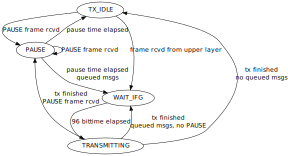
\includegraphics{figures/EtherMACFullDuplex_txstates}
\end{center}

The \nedtype{EtherMacFullDuplex} module records two scalars in addition to the
ones mentioned earlier:
\begin{itemize}
\item \ttt{rx channel idle (\%)}: reception channel idle time
        as a percentage of the total simulation time
\item \ttt{rx channel utilization (\%)}: total reception
        time as a percentage of the total simulation time
\end{itemize}

\subsection{EtherMac}

Ethernet MAC layer implementing CSMA/CD. It supports both half-duplex and full-duplex operations;
in full-duplex mode it behaves as \nedtype{EtherMacFullDuplex}. In half-duplex  mode
it detects collisions, sends jam messages and retransmit frames upon collisions using
the exponential backoff algorithm. In Gigabit Ethernet networks it supports carrier
extension and frame bursting. Carrier extension can be turned off by setting the
\fpar{carrierExtension} parameter to \ttt{false}.

Unlike \nedtype{EtherMacFullDuplex}, this MAC module processes the incoming packets when their
first bit is received. The end of the reception is calculated by the MAC and
detected by scheduling a self message.

When frames collide the transmission is aborted -- in this case the transmitting
station transmits a jam signal. Jam signals are represented
by a \msgtype{EtherJam} message. The jam message contains the tree identifier
of the frame whose transmission is aborted. When the \nedtype{EtherMac} receives a jam
signal, it knows that the corresponding transmission ended in jamming and have
been aborted. Thus when it receives as many jams as collided frames, it can
be sure that the channel is free again. (Receiving a jam message marks the
beginning of the jam signal, so actually has to wait for the duration of the jamming.)

The operation of the MAC module can be schematized by the following state chart:

\begin{center}
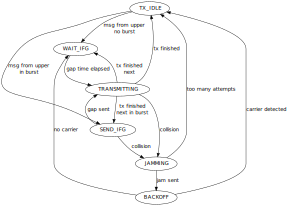
\includegraphics{figures/EtherMAC_txstates}
\end{center}

The module generates these extra signals:
\begin{itemize}
\item \fsignal{collision} when collision starts (received a frame,
         while transmitting or receiving another one; or start to transmit while receiving a frame),
         the constant value 1
\item \fsignal{backoff} when jamming period ended and before waiting according to the
         exponential backoff algorith, the constant value 1
\end{itemize}

These scalar statistics are generated about the state of the line:
\begin{itemize}
  \item \ttt{rx channel idle (\%)} reception channel idle time (full duplex) or channel
         idle time (half-duplex), as a percentage of the total simulation time
  \item \ttt{rx channel utilization (\%)} total successful reception time (full-duplex) or total
         successful reception/transmission time (half duplex), as a percentage
         of the total simulation time
  \item \ttt{rx channel collision (\%)} total unsuccessful reception time, as a percentage
         of the total simulation time
  \item \ttt{collisions} total number collisions (same as count of \fsignal{collisionSignal})
  \item \ttt{backoffs} total number of backoffs (same as count of \fsignal{backoffSignal})
\end{itemize}

\subsection{EtherEncap}

The \nedtype{EtherEncap} module generates \msgtype{EthernetIIFrame} messages.

EtherFrameII

\subsection{EtherLlc}

TODO what it does


% document error conditions (causing error() calls in the code)

% FIXME handleRestransmission() comment is not true: // no beginSendFrames(), because end of jam signal sending will trigger it automatically
%       in case of inner queue, the queued msg is not transmitted
% FIXME should not enter PAUSE state when !duplexMode


\section{Switches}

Ethernet switches play an important role in modern Ethernet LANs. Unlike
passive hubs and repeaters, that work in the physical layer, the switches
operate in the data link layer and routes data frames between the connected
subnets.

While a hub repeats the data frames on each connected line, possibly causing
collisions, switches help to segment the network to small collision domains.
In modern Gigabit LANs each node is connected to the switch direclty
by full-duplex lines, so no collisions are possible. In this case the
CSMA/CD is not needed and the channel utilization can be high.

\subsection{MAC relay units}

INET framework ethernet switches are built from \nedtype{IMacRelayUnit}
components. Each relay unit has N input and output gates for sending/receiving
Ethernet frames. They should be connected to \nedtype{IEtherMac} modules.

Internally the relay unit holds a table for the destination address -> output
port mapping. When it receives a data frame it updates the table with the
source address->input port. The table can also be pre-loaded from a text file
while initializing the relay unit. The file name given as the \fpar{addressTableFile}
parameter. Each line of the file contains a hexadecimal MAC address and a decimal port
number separated by tabs. Comment lines beginning with '\#' are also allowed:

\begin{verbatim}
01 ff ff ff ff    0
00-ff-ff-ee-d1    1
0A:AA:BC:DE:FF    2
\end{verbatim}

% FIXME #352 addressTableSize is not checked in readAddressTable -> if overflown
%            then later check updateTableWithAddress has no effect
% FIXME format is wrong in the comment of readAddressTable()

The size of the lookup table is restricted by the \fpar{addressTableSize} parameter.
When the table is full, the oldest address is deleted. Entries are also deleted
if their age exceeds the duration given as the \fpar{agingTime} parameter.

If the destination address is not found in the table, the frame is broadcasted.
The frame is not sent to the same subnet it was received from, because the
target already received the original frame. The only exception if the frame
arrived through a radio channel, in this case the target can be out of range.
The port range 0..\fpar{numWirelessPorts}-1 are reserved for wireless connections.

The \nedtype{IMacRelayUnit} module is not a concrete implementation,
it just defines gates and parameters an \nedtype{IMacRelayUnit} should have.
Concrete inplementations add
capacity and performance aspects to the model (number of frames processed
per second, amount of memory available in the switch, etc.)
C++ implementations can subclass from the class \cppclass{MACRelayUnitBase}.

There are two versions of \nedtype{IMacRelayUnit}:

\begin{description}
  \item[\nedtype{MACRelayUnitNP}] models one or more CPUs with shared memory,
    working from a single shared queue.
  \item[\nedtype{MACRelayUnitPP}] models one CPU assigned to each incoming port,
    working with shared memory but separate queues.
\end{description}

In both models input messages are queued. CPUs poll messages from the queue
and process them in \fpar{processingTime}. If the memory usage exceeds
\fpar{bufferSize}, the frame will be dropped.

A simple scheme for sending PAUSE frames is built in (although
users will probably change it). When the buffer level goes
above a high watermark, PAUSE frames are sent on all ports.
The watermark and the pause time is configurable; use zero
values to disable the PAUSE feature.

% FIXME valid values for pauseTime: 0..0xFFFF
% FIXME ETHER_PAUSE_COMMAND_BYTES should be 4 in Ethernet.h (2bytes opcode + 2bytes pauseTime)
% FIXME PAUSE frame should not be sent on all ports probably
% TODO add lowWatermark, send PauseFrame(pauseUnits=0) to resume sending

The relay units collects the following statistics:

\begin{description}
\item[usedBufferBytes] memory usage as function of time
\item[processedBytes] count and length of processed frames
\item[droppedBytes] count and length of frames dropped caused by out of memory
\end{description}

% FIXME MACRelayUnitNP: no signals are generated, how does @statistic work in the ned file?

\subsection{EtherSwitch}

Model of an Ethernet switch containing a relay unit and multiple MAC units.

The duplexChannel attributes of the MACs must be set according to the
medium connected to the port; if collisions are possible (it's a bus or hub)
it must be set to false, otherwise it can be set to true.
By default it uses half duples MAC with CSMA/CD.

TODO STP, RSTP



%%% Local Variables:
%%% mode: latex
%%% TeX-master: "usman"
%%% End:

\cleardoublepage

\chapter{The Radio Infrastructure}
\label{cha:radio}


\section{Overview}

Blah blah blah


%%% Local Variables:
%%% mode: latex
%%% TeX-master: "usman"
%%% End:


\cleardoublepage

\chapter{The 802.11 Model}
\label{cha:80211}


\section{Overview}

This chapter provides an overview of the IEEE 802.11 model for the INET Framework.

An IEEE 802.11 interface (NIC) comes in several flavours, differring
in their role (ad-hoc station, infrastructure mode station, or
access point) and their level of detail:

\begin{enumerate}
 \item \nedtype{Ieee80211Interface}: a generic (configurable) NIC
 \item \nedtype{Ieee80211NicAdhoc}: for ad-hoc mode
 \item \nedtype{Ieee80211NicAP}, \nedtype{Ieee80211NicAPSimplified}: for use in an access point
 \item \nedtype{Ieee80211NicSTA}, \nedtype{Ieee80211NicSTASimplified}: for use in an
   infrastructure-mode station
\end{enumerate}

NICs consist of four layers, which are the following (in top-down order):

\begin{enumerate}
  \item agent
  \item management
  \item MAC
  \item physical layer (radio)
\end{enumerate}

\textit{The physical layer} modules (\nedtype{Ieee80211Radio}) deal with modelling
transmission and reception of frames. They model the characteristics of
the radio channel, and determine if a frame was received correctly
(that is, it did not suffer bit errors due to low signal power or
interference in the radio channel). Frames received correctly are passed
up to the MAC. The implementation of these modules is based on the
Mobility Framework.

\textit{The MAC layer} (\nedtype{Ieee80211Mac}) performs transmission of frames according
to the CSMA/CA protocol. It receives data and management frames from
the upper layers, and transmits them.

\textit{The management layer} performs encapsulation and decapsulation of data packets
for the MAC, and exchanges management frames via the MAC with its peer
management entities in other STAs and APs. Beacon, Probe Request/Response,
Authentication, Association Request/Response etc frames are generated
and interpreted by management entities, and transmitted/received via
the MAC layer. During scanning, it is the management entity that periodically
switches channels, and collects information from received beacons and
probe responses.

The management layer has several implementations which differ in their role
(STA/AP/ad-hoc) and level of detail: \nedtype{Ieee80211MgmtAdhoc},
\nedtype{Ieee80211MgmtAp}, \nedtype{Ieee80211MgmtApSimplified}, \nedtype{Ieee80211MgmtSta},
\nedtype{Ieee80211MgmtStaSimplified}. The ..Simplified ones differ from the others
in that they do not model the scan-authenticate-associate process,
so they cannot be used in experiments involving handover.

\textit{The agent} is what instructs the management layer to perform
scanning, authentication and association. The management layer itself
just carries out these commands by performing the scanning, authentication
and association procedures, and reports back the results to the agent.

The agent layer is currenly only present in the \nedtype{Ieee80211NicSTA} NIC module,
as an \nedtype{Ieee80211AgentSta} module. The managament entities in other NIC
variants do not have as much freedom as to need an agent to control them.

By modifying or replacing the agent, one can alter the dynamic behaviour
of STAs in the network, for example implement different handover strategies.

\subsection{Limitations}

See the documentation of \nedtype{Ieee80211Mac} for features unsupported by this
model.

\ifdraft TODO
 further details about the implementation: what is modelled and what is
 not (beacons, auth, ...), communication between modules, frame formats,
 ...
\fi



%%% Local Variables:
%%% mode: latex
%%% TeX-master: "usman"
%%% End:


\cleardoublepage

\ifdraft TODO

\chapter{Node Mobility}
\label{cha:mobility}

\section{Mobility in INET}

\subsection{MobilityBase class}

The abstract \cppclass{MobilityBase} class is the base of the mobility
modules defined in the INET framework. This class implements things like
constraint area (or cubic volume), initial position, and border policy.

When the module is initialized it sets the initial position of the node
by calling the \ffunc{initializePosition()} method. The default implementation
handles the \fpar{initFromDisplayString}, \fpar{initialX}, \fpar{initialY}, \fpar{initialZ}
parameters.

The module is responsible for periodically updating the position.
For this purpose it should send timer messages to itself. These messages
are processed in the \ffunc{handleSelfMessage} method. In derived
classes, \ffunc{handleSelfMessage} should compute the new position
and update the display string and publish the new position by calling
the \ffunc{positionUpdated} method.

When the node reaches the boundary of the constraint area, the mobility
component has to prevent the node to exit. It can call the
\ffunc{handleIfOutside} method, which offers policies like
reflect, torus, random placement, and error.



\subsection{MovingMobilityBase}

The abstract \cppclass{MovingMobilityBase} class can be used to model
mobilities when the node moves on a continous trajectory and
updates its position periodically. Subclasses only need to implement
the \ffunc{move} method that is responsible to update the current
position and speed of the node.

The abstract \ffunc{move} method is called autmotically in every
\fpar{updateInterval} steps. The method is also called when a client
requested the current position or speed or when the \ffunc{move} method
requested an update at a future moment by setting the \fvar{nextChange}
field. This can be used when the state of the motion changes at a
specific time that is not a multiple of \fpar{updateInterval}.
The method can set the \fpar{stationary} field to \ttt{true} to
indicate that the node reached its final position and no more position
update is needed.

% TODO draw a plot of t-position function marking the points when
%      move() is called, stationary set to true, etc.

\subsection{LineSegmentsMobilityBase}

The path of a mobile node often consist of linear movements of constant
speed. The node moves with some speed for some time, then with another
speed for another duration and so on. If a mobility model fits this
description, it might be suitable to derive the implementing C++ class
from \cppclass{LineSegmentsMobilityBase}.

The module first choose a target position and a target time by calling
the \ffunc{setTargetPosition} method. If the target position differs
from the current position, it starts to move toward the target and
updates the position in the configured \fpar{updateInterval} intervals.
When the target position reached, it chooses a new target.

% TODO draw a plot like above, but containing linear segments, mark
%      the points when setTargetPosition called.

% FIXME LineSegmentsMobilityBase should not schedule the self message at updateInterval
%       when lastPosition==targetPosition (the node is waiting at the current position,
%       e.g. every second step in RandomWPMobility)
% TODO Consider an updateInterval computed from an updateDistance and speed, because position change
%      may be irrevelant during a preconfigured updateInterval.

\fi




\cleardoublepage

% based on 'integration' branch: 446a1265c28822456bc0230d362bbabdee7778ba (2012-03-19)

\chapter{IPv4}
\label{cha:ipv4}


\section{Overview}

The IP protocol is the workhorse protocol of the TCP/IP protocol suite.
All UDP, TCP, ICMP packets are encapsulated into IP datagrams and
transported by the IP layer.
While higher layer protocols transfer data among two communication end-point,
the IP layer provides an hop-by-hop, unreliable and connectionless delivery
service. IP does not maintain any state information about the individual
datagrams, each datagram handled independently.

The nodes that are connected to the Internet can be either a host or a router.
The hosts can send and recieve IP datagrams, and their operating system
implements the full TCP/IP stack including the transport layer. On the
other hand, routers have more than one interface cards and perform packet
routing between the connected networks. Routers does not need the
transport layer, they work on the IP level only. The division
between routers and hosts is not strict, because if a host
have several interfaces, they can usually be configured to operate
as a router too.

Each node on the Internet has a unique IP address. IP datagrams contain
the IP address of the destination. The task of the routers is to find
out the IP address of the next hop on the local network, and forward
the packet to it. Sometimes the datagram is larger, than the maximum
datagram that can be sent on the link (e.g. Ethernet has an 1500 bytes limit.).
In this case the datagram is split into fragments and each fragment is
transmitted independently. The destination host must collect all fragments,
and assemble the datagram, before sending up the data to the transport
layer.

\subsection{INET modules}

The INET framework contains several modules to build the
IPv4 network layer of hosts and routers:
\begin{itemize}
  \item \nedtype{IPv4} is the main module that implements RFC791. This
        module performs IP encapsulation/decapsulation, fragmentation
        and assembly, and routing of IP datagrams.
  \item The \nedtype{IPv4RoutingTable} is a helper module that manages the routing
        table of the node. It is queried by the \nedtype{IPv4} module
        for best routes, and updated by the routing daemons implementing
        RIP, OSPF, Manet, etc. protocols.
  \item The \nedtype{ICMP} module can be used to generate ICMP error packets. It also
        supports ICMP echo applications.
  \item The \nedtype{ARP} module performs the dynamic translation of IP addresses
        to MAC addresses.
  \item The \nedtype{IGMPv2} module to generate and process multicast group
        membership reports.
\end{itemize}

These modules are assembled into a complete network layer module
called \nedtype{IPv4NetworkLayer}. This module has
dedicated gates for TCP, UDP, SCTP, RSVP, OSPF, Manet, and Ping
higher layer protocols. It can be connected to several network
interface cards: Ethernet, PPP, Wlan, or external interfaces.
The \nedtype{IPv4NetworkLayer} module is used to build IPv4 hosts
(\nedtype{StandardHost}) and routers (\nedtype{Router}).

The implementation of these modules are based on the following RFCs:
\begin{itemize}
  \item RFC791: Internet Protocol
  \item RFC792: Internet Control Message Protocol
  \item RFC826: Address Resolution Protocol
  \item RFC1122: Requirements for Internet Hosts - Communication Layers
  \item RFC2236: Internet Group Management Protocol, Version 2
\end{itemize}

The subsequent sections describe the IPv4 modules in detail.

\section{The IPv4 Module}

The \nedtype{IPv4} module implements the IPv4 protocol.

For connecting the upper layer protocols the \nedtype{IPv4} module
has \emph{transportIn[]} and \emph{transportOut[]} gate vectors.

The IP packets are sent to the \nedtype{ARP} module through the
\emph{queueOut} gate. The incoming IP packets are received
directly from the network interface cards through the
\emph{queueIn[]} gates. Each interface card knows its own
network layer gate index.


\subsection{IP packets}

IP datagrams start with a variable length IP header.
The minimum length of the header is 20 bytes, and
it can contain at most 40 bytes for options, so
the maximum length of the IP header is 60 bytes.

\begin{center}
\begin{bytefield}{32}
\bitheader{0,3,4,7,8,15,16,18,19,23,24,31} \\
\bitbox{4}{Version} &
\bitbox{4}{IHL} &
\bitbox{8}{\small Type of Service} &
\bitbox{16}{Total Length} \\
\bitbox{16}{Identification} &
\bitbox{3}{Flags} &
\bitbox{13}{Fragment Offset} \\
\bitbox{8}{Time to Live} &
\bitbox{8}{Protocol} &
\bitbox{16}{Header Checksum} \\
\bitbox{32}{Source Address} \\
\bitbox{32}{Destination Address} \\
\bitbox{24}{Options} &
\bitbox{8}{Padding} \\
\end{bytefield}
\end{center}

The \ttt{Version} field is 4 for IPv4. The 4-bit \ttt{IHL} field is the
number of 32-bit words in the header. It is needed because the header
may contain optional fields, so its length may vary. The minimum IP header
length is 20, the maximum length is 60. The header is always padded to
multiple of 4 bytes. The \ttt{Type of Service} field designed to store
priority and preference values of the IP packet, so applications can
request low delay, high throughput, and maximium reliability from the
routing algorithms. In reality these fields are rarely set by applications,
and the routers mostly ignore them. The \ttt{Total Length} field is the
length of the whole datagram in bytes. The \ttt{Identification} field
is used for identifying the datagram sent by a host. It is usually generated
by incrementing a counter for each outgoing datagram. When the datagram
gets fragmented by a router, its \ttt{Identification} field is kept unchanged
to the other end can collect them. In datagram fragments the \ttt{Fragment Offset}
is the address of the fragment in the payload of the original datagram. It is
measured in 8-byte units, so fragment lengths must be a multiple of 8.
Each fragment except the last one, has its \ttt{MF} (more fragments) bit set
in the \ttt{Flags} field. The other used flag in \ttt{Flags} is the \ttt{DF}
(don't fragment) bit which forbids the fragmentation of the datagram.
The \ttt{Time to Live} field is decremented by each router in the path,
and the datagram is dropped if it reached 0. Its purpose is to prevent
endless cycles if the routing tables are not properly configured, but
can be used for limiting hop count range of the datagram (e.g. for local
broadcasts, but the \fprog{traceroute} program uses this field too).
The \ttt{Protocol} field is for demultiplexing the payload of the IP
datagram to higher level protocols. Each transport protocol has a registered
protocol identifier. The \ttt{Header Checksum} field is the 16-bit one's
complement sum of the header fields considered as a sequence of 16-bit numbers.
The \ttt{Source Address} and \ttt{Destination Address} are the IPv4 addresses
of the source and destination respectively.

The \ttt{Options} field contains 0 or more IP options. It is always padded
with zeros to a 32-bit boundary. An option is either a single-byte option
code or an option code + option length followed by the actual values for
the option. Thus IP implementations can skip unknown options.

An IP datagram is represented by the \msgtype{IPv4Datagram} message class.
It contains variables corresponding the fields of the IP header, except:
\begin{itemize}
  \item \fvar{Header Checksum} omitted, modeled by error bit of packets
  \item \fvar{Options} only the following options are permitted and the
                       datagram can contain at most one option:
        \begin{itemize}
          \item Loose Source Routing
          \item Strict Source Routing
          \item Timestamp
          \item Record Route
        \end{itemize}
\end{itemize}

The \fvar{Type of Service} field is called \ttt{diffServCodePoint} in
\nedtype{IPv4Datagram}.

Before sending the \msgtype{IPv4Datagram} through the network, the \nedtype{IPv4}
module attaches a \cppclass{IPv4RoutingDecision} control info.
The control info contains the IP address of the next hop, and the
identifier of the interface it should be sent. The ARP module translate
the IP address to the hardware address on the local net of the specified
interface and forwards the datagram to the interface card.


\subsection{Parameters}

The \nedtype{IPv4} module has the following parameters:
\begin{itemize}
  \item \fpar{procDelay} processing time of each incoming datagram.
  \item \fpar{timeToLive} default TTL of unicast datagrams.
  \item \fpar{multicastTimeToLive} default TTL of multicast datagrams.
  \item \fpar{protocolMapping} string value containing the \ttt{protocol id}
        $\rightarrow$ \ttt{gate index} mapping, e.g. \ttt{``6:0,17:1,1:2,2:3,46:4''}.
  \item \fpar{fragmentTimeout} the maximum duration until fragments are kept
          in the fragment buffer.
  \item \fpar{forceBroadcast} if \fkeyword{true}, then link-local broadcast
          datagrams are sent out through each interface, if the higher
          layer did not specify the outgoing interface.
\end{itemize}

% compile time options: WITH\_MANET, NEWFRAGMENT

\subsection{Statistics}

The \nedtype{IPv4} module does not write any statistics into files,
but it has some statistical information that can be watched during
the simulation in the gui environment.
\begin{itemize}
  \item \ttt{numForwarded}: number of forwarded datagrams, i.e. sent to one of the
        interfaces (not broadcast), counted before fragmentation.
  \item \ttt{numLocalDeliver}: number of datagrams locally delivered.
        (Each fragment counted separately.)
  \item \ttt{numMulticast}: number of routed multicast datagrams.
  \item \ttt{numDropped} number of dropped packets.
        Either because there is no any interface, the interface is not specified and
        no \fpar{forceBroadcast}, or received from the network but IP forwarding disabled.
  \item \ttt{numUnroutable}: number of unroutable datagrams, i.e. there is no
        route to the destination. (But if outgoing interface is specified it is routed!)
\end{itemize}

In the graphical interface the bubble of the \nedtype{IPv4} module
also displays these counters.


\section{The IPv4RoutingTable module}

The \nedtype{IPv4RoutingTable} module represents the routing table.
IP hosts and routers contain one instance of this class. It has
methods to manage the routing table and the interface table,
so one can achieve functionality similar to the \fprog{route} and
\fprog{ifconfig} commands.

This is a simple module without gates, it requires function calls to it
(message handling does nothing). Methods are provided for reading and
updating the interface table and the route table, as well as for unicast
and multicast routing.

\subsection*{Parameters}

The \nedtype{IPv4RoutingTable} module has the following parameters:

\begin{itemize}
  \item \fpar{routerId}: for routers, the router id using IPv4 address dotted notation;
        specify ``auto'' to select the highest interface address; should be left empty ``''
        for hosts
  \item \fpar{IPForward}: turns IP forwarding on/off (It is always \fkeyword{true}
                          in a \nedtype{Router} and is \fkeyword{false} by default
                          in a \nedtype{StandardHost}.)
  \item \fpar{forwardMulticast}: turns multicast IP forwarding on/off. Default is \fkeyword{false},
  should be set to \fkeyword{true} in multicast routers.
  \item \fpar{routingFile}: name of routing file that configures IP addresses and routes of the node
  containing this routing table. Its format is described in section \ref{subsec:routing_files}.
\end{itemize}

\begin{warning}
The \fpar{routingFile} parameter is obsolete. The prefered method for network configuration
is to use \nedtype{IPv4NetworkConfigurator}. The old config files should be replaced
with the XML configuration of \nedtype{IPv4NetworkConfigurator}. Section \ref{subsec:ipv4configurator}
describes the format of the new configuration files.
\end{warning}

% FIXME (#467) IPv4RoutingTable::invalidateCache() should clear localBroadcastAddresses.
% IPv4RoutingTable::findBestMatchingRoute() should search in this order:
%          1. host routes (exact match)
%          2. network routes (longest match)
%          3. default routes (round robin)
%   It is ok, if host routes has 255.255.255.255 netmask, and default has 0.0.0.0 netmask.
% FIXME IPv4RoutingTable::findBestMatchingRoute() if(...MANET...) branch always set bestRoute to NULL,
%       because if there were exact match, it would have been choosen in the previous loop.

\section{The ICMP module}

The Internet Control Message Protocol (ICMP) is the error reporting and
diagnostic mechanism of the Internet.
It uses the services of IP, so it is a transport layer protocol, but unlike
TCP or UDP it is not used to transfer user data. It can not be separated
from the IP, because the routing errors are reported by ICMP.

The \nedtype{ICMP} module can be used to send error messages and ping
request. It can also respond to incoming ICMP messages.

Each ICMP message is encapsulated within an IP datagram, so its delivery
is unreliable.

\begin{center}
\begin{bytefield}{32}
\bitheader{0,7,8,15,31} \\
\bitbox{8}{Type} &
\bitbox{8}{Code} &
\bitbox{16}{Checksum} \\
\bitbox{32}{Rest of header} \\
\wordbox{2}{Internet Header + 8 bytes of Original Datagram}
\end{bytefield}
\end{center}

The corresponding message class (\msgtype{ICMPMessage}) contains only
the Type and Code fields. The message encapsulates the IP packet that
triggered the error, or the data of the ping request/reply.

% FIXME type=PARAMETER_PROBLEM, code=0: missing Pointer field from ICMPMessage
%            REDIRECT: Gateway Internet Address
%            ECHO_REQUEST, ECHO_REPLY: Identifier, Sequence Number
%            TIMESTAMP_REQUEST, TIMESTAMP_REPLY: Identifier, Sequence Number, Originate Timestamp, Receive Timestamp, Transmit Timestamp

% FIXME wrong type codes for ICMP_DESTINATION_UNREACHABLE (3), ICMP_ECHO_REQUEST (8), ICMP_ECHO_REPLY (0), ICMP_TIMESTAMP_REQUEST (13), ICMP_TIMESTAMP_REPLY (14)

% FIXME ICMP header serializer handles only ICMP_ECHO_REQUEST, ICMP_ECHO_REPLY, ICMP_DESTINATION_UNREACHABLE, ICMP_TIME_EXCEEDED
%       ICMP header deserializer handles only ICMP_ECHO_REQUEST, ICMP_ECHO_REPLY

% FIXME ICMP error should not be send if the original datagram
%         1. is an ICMP error
%         2. was sent to a broadcast or multicast address
%         3. datagram was sent with a link-layer broadcast
%         4. a fragment other than the first
%         5. a datagram whose source address is 0.0.0.0, 127.*.*.*, broadcast or multicast address
%      currently only the 1. and half of 2. checked


% \section{The IGMP module}

\section{The ARP module}

The \nedtype{ARP} module implements the Address Resolution Protocol (RFC826).
The ARP protocol is designed to translate a local protocol address
to a hardware address. Altough the ARP protocol can be used with
several network protocol and hardware addressing schemes, in practice
they are almost always IPv4 and 802.3 addresses. The INET implementation
of the ARP protocol (the \nedtype{ARP} module) supports only
IP address $\rightarrow$ MAC address translation.

If a node wants to send an IP packet to a node whose MAC address is unknown,
it broadcasts an ARP frame on the Ethernet network.
In the request its publish its own IP and
MAC addresses, so each node in the local subnet can update their mapping.
The node whose MAC address was requested will respond with an ARP frame
containing its own MAC address directly to the node that sent the
request. When the original node receives the ARP response, it updates
its ARP cache and sends the delayed IP packet using the learned MAC address.

The frame format of the ARP request and reponse is shown in Figure \ref{fig:ARP_frame}.
In our case the HTYPE (hardware type), PTYPE (protocol type), HLEN (hardware address length)
and PLEN (protocol address length) are constants: HTYPE=Ethernet (1), PTYPE=IPv4 (2048), HLEN=6,
PLEN=4. The OPER (operation) field is 1 for an ARP request and 2 for an ARP response.
The SHA field contains the 48-bit hardware address of the sender, SPA field is
the 32-bit IP address of the sender; THA and TPA are the addresses of the target.
The message class corresponding to the ARP frame is \msgtype{ARPPacket}.
In this class only the OPER, SHA, SPA, THA and TPA fields are stored.
The length of an \msgtype{ARPPacket} is 28 bytes.

\begin{figure}[h]
\begin{center}
\label{fig:ARP_frame}
\begin{bytefield}{16}
\bitheader{0,7,8,15} \\
\bitbox{16}{HTYPE} \\
\bitbox{16}{PTYPE} \\
\bitbox{8}{HLEN} &
\bitbox{8}{PLEN} \\
\bitbox{16}{OPER} \\
\wordbox{3}{SHA} \\
\wordbox{2}{SPA} \\
\wordbox{3}{THA} \\
\wordbox{2}{TPA} \\
\end{bytefield}
\caption{ARP frame}
\end{center}
\end{figure}

The \nedtype{ARP} module receives IP datagrams and ARP responses from \nedtype{IPv4}
on the \ttt{ipIn} gate and transmits IP datagrams and ARP requests on the \ttt{nicOut[]} gates
towards the network interface cards. ARP broadcasts the requests on the local network,
so the NIC's entry in the \nedtype{InterfaceTable} should have \ffunc{isBroadcast()} flag
set in order to participate in the address resolution.

The incoming IP packet should have an attached \cppclass{IPv4RoutingDecision} control
info containing the IP address of the next hop. The next hop can be either an
IPv4 broadcast/multicast or a unicast address. The corresponding MAC addresses
can be computed for broadcast and multicast addresses (RFC 1122, 6.4); unicast
addresses are mapped using the ARP procotol.

If the hardware address is found
in the ARP cache, then the packet is transmitted to the addressed interface immediately.
Otherwise the packet is queued and an address resolution takes place.
The \nedtype{ARP} module creates an \msgtype{ARPPacket} object, sets the sender
MAC and IP address to its own address, sets the destination IP address
to the address of the target of the IP datagram, leave the destination MAC address
blank and broadcasts the packet on each network interface with broadcast capability.
Before sending the ARP packet, it retransmission a timer. If the timer expires,
it will retransmit the ARP request, until the maximum retry count is reached.
If there is no response to the ARP request, then the address resolution fails,
and the IP packet is dropped from the queue. Otherwise the MAC address of the
destination is learned and the IP packet can be transmitted on the corresponding
interface.

When an ARP packet is received on the \ttt{ipIn} gate, and the sender's IP
is already in the ARP cache, it is updated with the information in the ARP frame.
Then it is checked that the destination IP of the packet matches with our
address. In this case a new entry is created with the sender addresses in the
ARP cache, and if the packet is a request a response is created and sent directly
to the originator. If proxy ARP is enabled, the request can be responded
with our MAC address if we can route IP packets to the destination.

Usually each \nedtype{ARP} module maintains a local ARP cache.
However it is possible to use a global cache. The global cache is filled
in with entries of the IP and MAC addresses of the known interfaces
when the ARP modules are initiated (at simulation time 0).
\nedtype{ARP} modules that are using the global ARP cache
never initiate an address resolution; if an IP address not
found in the global cache, the simulation stops with an error.
However they will respond to ARP request, so the simulation can
be configured so that some \nedtype{ARP}s use local, while others
the global cache.

When an entry is inserted or updated in the local ARP cache,
the simulation time saved in the entry. The mapping in the
entry is not used after the configured \fpar{cacheTimeout}
elapsed. This parameter does not affect the entries of
the global cache however.

The module parameters of \nedtype{ARP} are:

\begin{itemize}
  \item \fpar{retryTimeout}: number of seconds ARP waits between retries to resolve an IPv4 address (default is 1s)
  \item \fpar{retryCount}: number of times ARP will attempt to resolve an IPv4 address (default is 3)
  \item \fpar{cacheTimeout}: number of seconds unused entries in the cache will time out (default is 120s)
  \item \fpar{proxyARP}: enables proxy ARP mode (default is \fkeyword{true})
  \item \fpar{globalARP}: use global ARP cache (default is \fkeyword{false})
\end{itemize}

The \nedtype{ARP} module emits four signals:

\begin{itemize}
  \item \ttt{sentReq}: emits 1 each time an ARP request is sent
  \item \ttt{sentReplies}: emits 1 each time an ARP response is sent
  \item \ttt{initiatedResolution}: emits 1 each time an ARP resolution is initiated
  \item \ttt{failedResolution}: emits 1 each time an ARP resolution is failed
\end{itemize}

These signals are recorded as vectors and their counts as scalars.

% TODO watches, animation effects

\section{The IGMP module}

The IGMP module is responsible for distributing the information of
multicast group memberships from hosts to routers. When an interface
of a host joins to a multicast group, it will send an IGMP report
on that interface to routers. It can also send reports when the
interface leaves the multicast group, so it does not want to
receive those multicast datagrams. The IGMP module of multicast
routers processes these IGMP reports: it updates the list of
groups, that has members on the link of the incoming message.

The \nedtype{IIGMP} module interface defines the connections
of IGMP modules.
IGMP reports are transmitted by IP, so the module contains
gates to be connected to the IP module (\ttt{ipIn/ipOut}). The IP
module delivers packets with protocol number 2 to the IGMP module.
However some multicast routing protocols (like DVMRP) also exchange
routing information by sending IGMP messages, so they should be
connected to the \ttt{routerIn/routerOut} gates of the IGMP module.
The IGMP module delivers the IGMP messages not processed by itself
to the connected routing module.

The \nedtype{IGMPv2} module implements version 2 of the IGMP protocol
(RFC 2236). Next we describe its behaviour in host and routers in details.
Note that multicast routers behaves as hosts too, i.e. they are sending
reports to other routers when joining or leaving a multicast group.

\subsection{Host behaviour}

When an interface joins to a multicast group, the host
will send a Membership Report immediately to the group address.
This report is repeated after \fpar{unsolicetedReportInterval} to
cover the possibility of the first report being lost.

When a host's interface leaves a multicast group, and it was
the last host that sent a Membership Report for that group,
it will send a Leave Group message to the all-routers multicast
group (224.0.0.2).

This module also responds to IGMP Queries. When the host
receives a Group-Specific Query on an interface that belongs
to that group, then it will set a timer to a random value
between 0 and Max Response Time of the Query. If the timer
expires before the host observe a Membership Report sent
by other hosts, then the host sends an IGMPv2 Membership Report.
When the host receives a General Query on an interface,
a timer is initialized and a report is sent for each group
membership of the interface.

\subsection{Router behaviour}

Multicast routers maintains a list for each interface containing
the multicast groups that have listeners on that interface.
This list is updated when IGMP Membership Reports and Leave Group
messages arrive, or when a timer expires since the last Query.

When multiple routers are connected to the same link, the one with
the smallest IP address will be the Querier. When other routers
observe that they are Non-Queriers (by receiving an IGMP Query
with a lower source address), they stop sending IGMP Queries
until \fpar{otherQuerierPresentInterval} elapsed since the last
received query.

Routers periodically (\fpar{queryInterval}) send a General Query
on each attached network for which this router is a Querier.
On startup the router sends \fpar{startupQueryCount} queries
separated by \fpar{startupQueryInterval}. A General Query
has unspecified Group Address field, a Max Response Time
field set to \fpar{queryResponseInterval}, and is sent to the
all-systems multicast address (224.0.0.1).

When a router receives a Membership Report, it will add the
reported group to the list of multicast group memberships.
At the same time it will set a timer for the membership
to \fpar{groupMembershipInterval}. Repeated reports restart
the timer. If the timer expires, the router assumes
that the group has no local members, and multicast traffic
is no more forwarded to that interface.

When a Querier receives a Leave Group message for a group,
it sends a Group-Specific Query to the group being left.
It repeats the Query \fpar{lastMemberQueryCount} times in
separated by \fpar{lastMemberQueryInterval} until a Membership
Report is received. If no Report received, then the router
assumes that the group has no local members.

% FIXME IGMPv2 not compatible with IGMPv1 hosts and routers

\subsection{Disabling IGMP}

The IPv4 \nedtype{IPv4NetworkLayer} contains an instance of the IGMP
module. IGMP can be turned off by setting the \fpar{enabled}
parameter to false. When disabled, then no IGMP message
is generated, and incoming IGMP messages are ignored.

\subsection{Parameters}

The following parameters has effects in both hosts and routers:

\begin{itemize}
  \item \fpar{enabled} if \fkeyword{false} then the IGMP module is silent. Default is \fkeyword{true}.
\end{itemize}

These parameters are only used in hosts:

\begin{itemize}
  \item \fpar{unsolicitedReportInterval} the time between repetitions of a
   host's initial report of membership in a group. Default is 10s.
\end{itemize}

Router timeouts are configured by these parameters:

\begin{itemize}
  \item \fpar{robustnessVariable} the IGMP is robust to \fpar{robustnessVariable}-1
   packet losses. Default is 2.
  \item \fpar{queryInterval} the interval between General Queries sent by a Querier.
   Default is 125s.
  \item \fpar{queryResponseInterval} the Max Response Time inserted into General Queries
  \item \fpar{groupMembershipInterval} the amount of time that must pass before
   a multicast router decides there are no more members of a group on a network.
   Fixed to \fpar{robustnessVariable} * \fpar{queryInterval} + \fpar{queryResponseInterval}.
  \item \fpar{otherQuerierPresentInterval} the length of time that must
   pass before a multicast router decides that there is no longer
   another multicast router which should be the querier.
   Fixed to \fpar{robustnessVariable} * \fpar{queryInterval} + \fpar{queryResponseInterval} / 2.
  \item \fpar{startupQueryInterval} the interval between General Queries
   sent by a Querier on startup. Default is \fpar{queryInterval} / 4.
  \item \fpar{startupQueryCount} the number of Queries sent out on startup,
   separated by the \fpar{startupQueryInterval}. Default is \fpar{robustnessVariable}.
  \item \fpar{lastMemberQueryInterval} the Max Response Time inserted into
   Group-Specific Queries sent in response to Leave Group messages, and
   is also the amount of time between Group-Specific Query messages.
   Default is 1s.
  \item \fpar{lastMemberQueryCount} the number of Group-Specific Queries
   sent before the router assumes there are no local members.
   Default is \fpar{robustnessVariable}.
\end{itemize}

\section{The IPv4NetworkLayer module}

The \nedtype{IPv4NetworkLayer} module packs the \nedtype{IP}, \nedtype{ICMP},
\nedtype{ARP}, and \nedtype{IGMP} modules into one compound module.
The compound module defines gates for connecting UDP, TCP, SCTP, RSVP and
OSPF transport protocols. The \ttt{pingIn} and \ttt{pingOut} gates of the
\nedtype{ICMP} module are also available, while its \ttt{errorOut} gate
is connected to an inner \nedtype{ErrorHandling} component that writes
the ICMP errors to the log.

The component can be used in hosts and routers to support IPv4.

\section{The NetworkInfo module}

The \nedtype{NetworkInfo} module can be used to dump detailed information
about the network layer. This module does not send or received messages,
it is invoked by the \nedtype{ScenarioManager} instead. For example
the following \nedtype{ScenarioManager} script dump the routing table
of the \ttt{LSR2} module at simulation time $t=2$ into \ffilename{LSR2\_002.txt}:
\begin{filelisting}
<scenario>
  <at t="2">
    <routing module="NetworkInfo" target="LSR2" file="LSR2_002.txt"/>
  </at>
</scenario>
\end{filelisting}

The module currently support only the \ttt{routing} command which dumps
the routing table. The command has four parameters given as XML attributes:
\begin{itemize}
  \item \ttt{target} the name of the node that owns the routing table to be dumped
  \item \ttt{filename} the name of the file the output is directed to
  \item \ttt{mode} if set to ``a'', the output is appended to the file,
                   otherwise the target is truncated if the file existed
  \item \ttt{compat} if set to ``linux'', then the output is generated
                     in the format of the \ttt{route -n} command of Linux.
                     The output is sorted only if \ttt{compat} is
                     \fkeyword{true}.
\end{itemize}

\section{Configuring IPv4 networks}

An IPv4 network is composed of several nodes like hosts, routers,
switches, hubs, Ethernet buses, or wireless access points.
The nodes having a IPv4 network layer (hosts and routers) should be
configured at the beginning of the simulation. The configuration
assigns IP addresses to the nodes, and fills their routing tables.
If multicast forwarding is simulated, then the multicast routing
tables also must be filled in.

% TODO define nodes, IP nodes, routers, multicast routers

The configuration can be manual (each address and route is fully specified
by the user), or automatic (addresses and routes are generated by
a configurator module at startup).

Before version 1.99.4 INET offered \nedtype{FlatNetworkConfigurator}
for automatic and routing files for manual configuration.
Both had serious limitations, so a new configurator has been added
in version 1.99.4: \nedtype{IPv4NetworkConfigurator}. This configurator
supports both fully manual and fully automatic configuration. It
can also be used with partially specified manual configurations,
the configurator fills in the gaps automatically.

The next section describes the usage of \nedtype{IPv4NetworkConfigurator},
\nedtype{FlatNetworkConfigurator} and old routing files are described
in the following sections.

\subsection{IPv4NetworkConfigurator}
\label{subsec:ipv4configurator}

The \nedtype{IPv4NetworkConfigurator} assigns IP addresses and sets up
static routing for an IPv4 network.

It assigns per-interface IP addresses, strives to take subnets into account,
and can also optimize the generated routing tables by merging routing entries.

Hierarchical routing can be set up by using only a fraction of configuration
entries compared to the number of nodes. The configurator also does
routing table optimization that significantly decreases the size of routing
tables in large networks.

The configuration is performed in stage 2 of the initialization. At this
point interface modules (e.g. PPP) has already registered their interface
in the interface table. If an interface is named \ttt{ppp[0]}, then the
corresponding interface entry is named \ttt{ppp0}. This name can be used
in the config file to refer to the interface.

The configurator goes through the following steps:
\begin{enumerate}
  \item  Builds a graph representing the network topology. The graph
     will have a vertex for every module that has a @node property (this
     includes hosts, routers, and L2 devices like switches, access points,
     Ethernet hubs, etc.) It also assigns weights to vertices and edges that
     will be used by the shortest path algorithm when setting up routes.
     Weights will be infinite for IP nodes that have IP forwarding disabled
     (to prevent routes from transiting them), and zero for all other nodes
     (routers and and L2 devices). Edge weights are chosen to be inversely
     proportional to the bitrate of the link, so that the configurator
     prefers connections with higher bandwidth. For internal purposes,
     the configurator also builds a table of all "links" (the link data
     structure consists of the set of network interfaces that are
     on the same point-to-point link or LAN)

  \item  Assigns IP addresses to all interfaces of all nodes. The
     assignment process takes into consideration the addresses and netmasks
     already present on the interfaces (possibly set in earlier initialize
     stages), and the configuration provided in the XML format (described
     below). The configuration can specify "templates" for the address
     and netmask, with parts that are fixed and parts that can be chosen
     by the configurator (e.g. "10.0.x.x"). In the most general case,
     the configurator is allowed to choose any address and netmask for all
     interfaces (which results in automatic address assignment). In the most
     constrained case, the configurator is forced to use the requested addresses
     and netmasks for all interfaces (which translates to manual address assignment).
     There are many possible configuration options between these two extremums. The
     configurator assigns addresses in a way that maximizes the number of
     nodes per subnet. Once it figures out the nodes that belong to a single
     subnet it, will optimize for allocating the longest possible netmask.
     The configurator might fail to assign netmasks and addresses according
     to the given configuration parameters; if that happens, the assignment
     process stops and an error is signalled.

  \item  Adds the manual routes that are specified in the configuration.

  \item  Adds static routes to all routing tables in the network. The
     configurator uses Dijkstra's weighted shortest path algorithm to find
     the desired routes between all possible node pairs. The resulting
     routing tables will have one entry for all destination interfaces in the
     network. The configurator can be safely instructed to add default routes
     where applicable, significantly reducing the size of the host routing
     tables. It can also add subnet routes instead of interface routes further
     reducing the size of routing tables. Turning on this option requires
     careful design to avoid having IP addresses from the same subnet on
     different links. CAVEAT: Using manual routes and static route generation
     together may have unwanted side effects, because route generation ignores
     manual routes.

  \item  Then it optimizes the routing tables for size. This optimization allows
     configuring larger networks with smaller memory footprint and makes the
     routing table lookup faster. The resulting routing table might be
     different in that it will route packets that the original routing table
     did not. Nevertheless the following invariant holds: any packet routed
     by the original routing table (has matching route) will still be routed
     the same way by the optimized routing table.

  \item  Finally it dumps the requested results of the configuration. It can
     dump network topology, assigned IP addresses, routing tables and its
     own configuration format.
\end{enumerate}

The module can dump the result of the configuration in the XML format
which it can read. This is useful to save the result of a time consuming
configuration (large network with optimized routes), and use it as
the config file of subsequent runs.

\subsubsection*{Network topology graph}

The network topology graph is constructed from the nodes
of the network. The node is a module having a @node property
(this includes hosts, routers, and L2 devices like switches,
 access points, Ethernet hubs, etc.). An IP node is a node
that contains an \nedtype{InterfaceTable} and a \nedtype{IPv4RoutingTable}.
A router is an IP node that has multiple network interfaces,
and IP forwarding is enabled in its routing table module.
In multicast routers the \fpar{forwardMulticast} parameter
is also set to \fkeyword{true}.

A link is a set of interfaces that can send datagrams to each other
without intervening routers. Each interface belongs to exactly
one link. For example two interface connected
by a point-to-point connection forms a link. Ethernet interfaces
connected via buses, hubs or switches.
The configurator identifies links by discovering
the connections between the IP nodes, buses, hubs, and switches.

Wireless links are identified by the \fpar{ssid} or \fpar{accessPointAddress}
parameter of the 802.11 management module. Wireless interfaces
whose node does not contain a management module are supposed
to be on the same wireless link. Wireless links can also be
configured in the configuration file of \nedtype{IPv4NetworkConfigurator}:
\begin{verbatim}
<config>
  <wireless hosts="area1.*" interfaces="wlan*">
</config>
\end{verbatim}
puts wlan interfaces of the specified hosts into the same wireless link.

If a link contains only one router, it is marked as the gateway
of the link. Each datagram whose destination is outside the link
must go through the gateway.

\subsubsection*{Address assignment}

Addresses can be set up manually by giving the address and netmask for
each IP node. If some part of the address or netmask is unspecified,
then the configurator can fill them automatically. Unspecified fields
are given as an ``x'' character in the dotted notation of the address.
For example, if the address is specified as 192.168.1.1 and the
netmask is 255.255.255.0, then the node address will be 192.168.1.1
and its subnet is 192.168.1.0. If it is given as 192.168.x.x and
255.255.x.x, then the configurator chooses a subnet address in the range
of 192.168.0.0 - 192.168.255.252, and an IP address within the chosen
subnet. (The maximum subnet mask is 255.255.255.252 allows 2 nodes in the subnet.)

The following configuration generates network addresses below the 10.0.0.0
address for each link, and assign unique IP addresses to each host:

\begin{verbatim}
<config>
  <interface hosts="*" address="10.x.x.x" netmask="255.x.x.x"/>
</config>
\end{verbatim}

The configurator tries to put nodes on the same link into the same subnet,
so its enough to configure the address of only one node on each link.

The following example configures a hierarchical network in a way that keeps
routing tables small.
\begin{verbatim}
<config>
  <interface hosts="area11.lan1.*" address="10.11.1.x" netmask="255.255.255.x"/>
  <interface hosts="area11.lan2.*" address="10.11.2.x" netmask="255.255.255.x"/>
  <interface hosts="area12.lan1.*" address="10.12.1.x" netmask="255.255.255.x"/>
  <interface hosts="area12.lan2.*" address="10.12.2.x" netmask="255.255.255.x"/>
  <interface hosts="area*.router*" address="10.x.x.x" netmask="x.x.x.x"/>
  <interface hosts="*" address="10.x.x.x" netmask="255.x.x.0"/>
</config>
\end{verbatim}

The XML configuration must contain exactly one \verb!<config>! element. Under the
root element there can be multiple of the following elements:

The interface element provides configuration parameters for one or more
interfaces in the network. The selector attributes limit the scope where
the interface element has effects. The parameter attributes limit the
range of assignable addresses and netmasks.
The \verb!<interface>! element may contain the following attributes:
\begin{compactitem}
    \item \ttt{@hosts}
      Optional selector attribute that specifies a list of host name patterns.
      Only interfaces in the specified hosts are affected. The pattern might
      be a full path starting from the network, or a module name anywhere in
      the hierarchy, and other patterns similar to ini file keys. The default
      value is "*" that matches all hosts.
      e.g. "subnet.client*" or "host* router[0..3]" or "area*.*.host[0]"

    \item \ttt{@names}
      Optional selector attribute that specifies a list of interface name
      patterns. Only interfaces with the specified names are affected. The
      default value is "*" that matches all interfaces.
      e.g. "eth* ppp0" or "*"

    \item \ttt{@towards}
      Optional selector attribute that specifies a list of host name patterns.
      Only interfaces connected towards the specified hosts are affected. The
      specified name will be matched against the names of hosts that are on
      the same LAN with the one that is being configured. This works even if
      there's a switch between the configured host and the one specified here.
      For wired networks it might be easier to specify this parameter instead
      of specifying the interface names. The default value is "*".
      e.g. "ap" or "server" or "client*"

    \item \ttt{@among}
      Optional selector attribute that specifies a list of host name patterns.
      Only interfaces in the specified hosts connected towards the specified
      hosts are affected.
      The 'among="X Y Z"' is same as 'hosts="X Y Z" towards="X Y Z"'.

    \item \ttt{@address}
      Optional parameter attribute that limits the range of assignable
      addresses. Wildcards are allowed with using 'x' as part of the address
      in place of a byte. Unspecified parts will be filled automatically by
      the configurator. The default value "" means that the address will not
      be configured. Unconfigured interfaces still have allocated addresses
      in their subnets allowing them to become configured later very easily.
      e.g. "192.168.1.1" or "10.0.x.x"

    \item \ttt{@netmask}
      Optional parameter attribute that limits the range of assignable
      netmasks. Wildcards are allowed with using 'x' as part of the netmask
      in place of a byte. Unspecified parts will be filled automatically be
      the configurator. The default value "" means that any netmask can be
      configured.
      e.g. "255.255.255.0" or "255.255.x.x" or "255.255.x.0"

    \item \ttt{@mtu}                number
      Optional parameter attribute to set the MTU parameter in the interface.
      When unspecified the interface parameter is left unchanged.

    \item \ttt{@metric}                number
      Optional parameter attribute to set the Metric parameter in the interface.
      When unspecified the interface parameter is left unchanged.
\end{compactitem}

Wireless interfaces can similarly be configured by adding
\verb!<wireless>! elements to the configuration. Each \verb!<wireless>!
element with a different id defines a separate subnet.
\begin{compactitem}
    \item \ttt{@id} (optional)
      identifies wireless network, unique value used if missed

    \item \ttt{@hosts}
      Optional selector attribute that specifies a list of host name patterns.
      Only interfaces in the specified hosts are affected. The default value
      is "*" that matches all hosts.

    \item \ttt{@interfaces}
      Optional selector attribute that specifies a list of interface name
      patterns. Only interfaces with the specified names are affected. The
      default value is "*" that matches all interfaces.
\end{compactitem}


\subsubsection{Multicast groups}

Multicast groups can be configured by adding \verb!<multicast-group>!
elements to the configuration file. Interfaces belongs to a multicast
group will join to the group automatically.

For example
\begin{verbatim}
<config>
  <multicast-group hosts="router*" interfaces="eth*" address="224.0.0.5"/>
</config>
\end{verbatim}
adds all Ethernet interfaces of nodes whose name starts with ``router''
to the 224.0.0.5 multicast group.

The \verb!<multicast-group>! element has the following attributes:
\begin{compactitem}
    \item \ttt{@hosts}
      Optional selector attribute that specifies a list of host name patterns.
      Only interfaces in the specified hosts are affected. The default value
      is "*" that matches all hosts.

    \item \ttt{@interfaces}
      Optional selector attribute that specifies a list of interface name
      patterns. Only interfaces with the specified names are affected. The
      default value is "*" that matches all interfaces.

    \item \ttt{@towards}
      Optional selector attribute that specifies a list of host name patterns.
      Only interfaces connected towards the specified hosts are affected.
      The default value is "*".

    \item \ttt{@among}
      Optional selector attribute that specifies a list of host name patterns.
      Only interfaces in the specified hosts connected towards the specified
      hosts are affected.
      The 'among="X Y Z"' is same as 'hosts="X Y Z" towards="X Y Z"'.

    \item \ttt{@address}
      Mandatory parameter attribute that specifies a list of multicast group
      addresses to be assigned. Values must be selected from the valid range
      of multicast addresses.
      e.g. "224.0.0.1 224.0.1.33"
\end{compactitem}


\subsubsection*{Manual route configuration}

The \nedtype{IPv4NetworkConfigurator} module allows the user
to fully specify the routing tables of IP nodes at the beginning
of the simulation.

The \verb!<route>! elements of the configuration add a route to the
routing tables of selected nodes. The element has the following attributes:
\begin{compactitem}
    \item \ttt{@hosts}
      Optional selector attribute that specifies a list of host name patterns.
      Only routing tables in the specified hosts are affected. The default
      value "" means all hosts will be affected.
      e.g. "host* router[0..3]"

    \item \ttt{@destination}
      Optional parameter attribute that specifies the destination address in
      the route (L3AddressResolver syntax). The default value is "*".
      e.g. "192.168.1.1" or "subnet.client[3]" or "subnet.server(ipv4)" or "*"

    \item \ttt{@netmask}
      Optional parameter attribute that specifies the netmask in the route.
      The default value is "*".
      e.g. "255.255.255.0" or "/29" or "*"

    \item \ttt{@gateway}
      Optional parameter attribute that specifies the gateway (next-hop)
      address in the route (L3AddressResolver syntax). When unspecified
      the interface parameter must be specified. The default value is "*".
      e.g. "192.168.1.254" or "subnet.router" or "*"

    \item \ttt{@interface}
      Optional parameter attribute that specifies the output interface name
      in the route. When unspecified the gateway parameter must be specified.
      This parameter has no default value.
      e.g. "eth0"

    \item \ttt{@metric}
      Optional parameter attribute that specifies the metric in the route.
      The default value is 0.
\end{compactitem}

Multicast routing tables can similarly be configured by adding
\verb!<multicast-route>! elements to the configuration.
\begin{compactitem}
    \item \ttt{@hosts}
      Optional selector attribute that specifies a list of host name patterns.
      Only routing tables in the specified hosts are affected.
      e.g. "host* router[0..3]"

    \item \ttt{@source}
      Optional parameter attribute that specifies the address of the source
      network. The default value is "*" that matches all sources.

    \item \ttt{@netmask}
      Optional parameter attribute that specifies the netmask of the source
      network. The default value is "*" that matches all sources.

    \item \ttt{@groups}
      Optional List of IPv4 multicast addresses specifying the groups this entry
      applies to. The default value is "*" that matches all multicast groups.
      e.g. "225.0.0.1 225.0.1.2".

    \item \ttt{@metric}
      Optional parameter attribute that specifies the metric in the route.

    \item \ttt{@parent}
      Optional parameter attribute that specifies the name of the interface
      the multicast datagrams are expected to arrive. When a datagram arrives
      on the parent interface, it will be forwarded towards the child interfaces;
      otherwise it will be dropped. The default value is the interface on the
      shortest path towards the source of the datagram.

    \item \ttt{@children}
      Mandatory parameter attribute that specifies a list of interface name
      patterns:
      \begin{compactitem}
        \item a name pattern (e.g. "ppp*") matches the name of the interface
        \item a 'towards' pattern (starting with ">", e.g. ">router*") matches the interface
         by naming one of the neighbour nodes on its link.
      \end{compactitem}
      Incoming multicast datagrams are forwarded to each child interface except the
      one they arrived in.
\end{compactitem}

The following example adds an entry to the multicast routing table of \ttt{router1},
that intsructs the routing algorithm to forward multicast datagrams whose source
is in the 10.0.1.0 network and whose destinatation address is 225.0.0.1 to
send on the \ttt{eth1} and \ttt{eth2} interfaces assuming it arrived on the
\ttt{eth0} interface:

\begin{verbatim}
<multicast-route hosts="router1" source="10.0.1.0" netmask="255.255.255.0"
                 groups="225.0.0.1" metric="10"
                 parent="eth0" children="eth1 eth2"/>
\end{verbatim}

\subsubsection*{Automatic route configuration}

If the \fpar{addStaticRoutes} parameter is true, then
the configurator add static routes to all routing tables.

The configurator uses Dijkstra's weighted shortest path algorithm to find
the desired routes between all possible node pairs. The resulting
routing tables will have one entry for all destination interfaces in the
network.

%     Weights will be infinite for IP nodes that have IP forwarding disabled
%     (to prevent routes from transiting them), and zero for all other nodes
%     (routers and and L2 devices). Edge weights are chosen to be inversely
%     proportional to the bitrate of the link, so that the configurator
%     prefers connections with higher bandwidth. For internal purposes,

The configurator can be safely instructed to add default routes
where applicable, significantly reducing the size of the host routing
tables. It can also add subnet routes instead of interface routes further
reducing the size of routing tables. Turning on this option requires
careful design to avoid having IP addresses from the same subnet on
different links.


\begin{caution}
Using manual routes and static route generation
together may have unwanted side effects, because route generation ignores
manual routes. Therefore if the configuration file contains
manual routes, then the \fpar{addStaticRoutes} parameter should be set
to \fkeyword{false}.
\end{caution}

\subsubsection*{Route optimization}

If the \fpar{optimizeRoutes} parameter is \fkeyword{true} then the
configurator tries to optimize the routing table for size.
This optimization allows configuring larger networks with smaller
memory footprint and makes the routing table lookup faster.

The optimization is performed by merging routes whose gateway and
outgoing interface is the same by finding a common prefix that
matches only those routes. The resulting routing table might be
different in that it will route packets that the original routing table
did not. Nevertheless the following invariant holds: any packet routed
by the original routing table (has matching route) will still be routed
the same way by the optimized routing table.

\subsubsection*{Parameters}

This list summarize the parameters of the \nedtype{IPv4NetorkConfigurator}:

\begin{params}
  \param{config}
   {XML configuration parameters for IP address assignment and adding manual routes.}
  \param{assignAddresses}
   {assign IP addresses to all interfaces in the network}
  \param{assignDisjunctSubnetAddresses}
   {avoid using the same address prefix and
    netmask on different links when assigning IP addresses to interfaces}
  \param{addStaticRoutes}
   {add static routes to the routing tables of all nodes
    to route to all destination interfaces (only where applicable; turn off when
    config file contains manual routes)}
  \param{addDefaultRoutes}
    {add default routes if all routes from a source node go
     through the same gateway (used only if addStaticRoutes is true)}
  \param{addSubnetRoutes}
   {add subnet routes instead of destination interface routes
    (only where applicable; used only if addStaticRoutes is true)}
  \param{optimizeRoutes}
   {optimize routing tables by merging routes, the resulting routing table might
    route more packets than the original (used only if addStaticRoutes is true)}
  \param{dumpTopology}
   {if true, then the module prints extracted network topology}
  \param{dumpAddresses}
   {if true, then the module prints assigned IP addresses for all interfaces}
  \param{dumpRoutes}
   {if true, then the module prints configured and optimized routing tables for all nodes to
    the module output}
  \param{dumpConfig}
   {name of the file, write configuration into the given config file that can be fed back
    to speed up subsequent runs (network configurations)}
\end{params}

\subsection{FlatNetworkConfigurator}

The \nedtype{FlatNetworkConfigurator} module configures
IP addresses and routes of IP nodes of a network.
All assigned addresses share a common subnet prefix,
the network topology will be ignored. Shortest path
routes are also generated from any node to any other
node of the network. The Gateway (next hop) field of the routes
is not filled in by these configurator, so it relies
on proxy ARP if the network spans several LANs.

% no optimization of routing tables

The \nedtype{FlatNetworkConfigurator} module configures
the network when it is initialized. The configuration
is performed in stage 2, after interface tables are
filled in. Do not use a \nedtype{FlatNetworkConfigurator}
module together with static routing files, because they
can iterfere with the configurator.

The \nedtype{FlatNetworkConfigurator} searches each IP nodes of the network.
(IP nodes are those modules that have the @node NED property and
has a \nedtype{IPv4RoutingTable} submodule named ``routingTable'').
The configurator then assigns IP addresses to the IP nodes, controlled
by the following module parameters:
\begin{itemize}
  \item \fpar{netmask} common netmask of the addresses (default is 255.255.0.0)
  \item \fpar{networkAddress} higher bits are the network part of the addresses,
        lower bits should be 0. (default is 192.168.0.0)
\end{itemize}

With the default parameters the assigned addresses are in the range
192.168.0.1 - 192.168.255.254, so there can be maximum 65534 nodes in the
network. The same IP address will be assigned to each interface
of the node, except the loopback interface which always has address 127.0.0.1
(with 255.0.0.0 mask).

After assigning the IP addresses, the configurator fills in the routing tables.
There are two kind of routes:
\begin{itemize}
  \item default routes: for nodes that has only one non-loopback interface
        a route is added that matches with any destination address
        (the entry has 0.0.0.0 \ttt{host} and \ttt{netmask} fields).
        These are remote routes, but the gateway address is left unspecified.
        The delivery of the datagrams rely on the proxy ARP feature of the
        routers.
  \item direct routes following the shortest paths: for nodes that has more
        than one non-loopback interface a separate route is added to each
        IP node of the network. The outgoing interface is chosen by the
        shortest path to the target node. These routes are
        added as direct routes, even if there is no direct link with the
        destination. In this case proxy ARP is needed to deliver the datagrams.
\end{itemize}

\begin{note}
This configurator does not try to optimize the routing tables.
If the network contains $n$ nodes, the size of all routing tables
will be proportional to $n^2$, and the time of the lookup of the
best matching route will be proportional to $n$.
\end{note}

% FIXME weird FlatNetworkConfigurator behaviour.
%       Assigned IP addresses does not mirror the hierachy of networks (e.g. each node in an Ethernet LAN handled as a one-element subnet).
%       No gateway address is set in the routes, delivery relies on proxy ARPing.
%       Direct routes created to each node, even if there is no direct link to it.
%       Different interfaces of a node should have different IP address.
%       Broadcast capable interfaces should have a real netmast (not 255.255.255.255) to support subnet directed IP broadcasts.

\subsection{Old routing files}
\label{subsec:routing_files}

Routing files are files with \ttt{.irt} or \ttt{.mrt} extension,
and their names are passed in the \fpar{routingFile} parameter
to \nedtype{IPv4RoutingTable} modules.

Routing files may contain network interface configuration and static
routes. Both are optional. Network interface entries in the file
configure existing interfaces; static routes are added to the route table.

Interfaces themselves are represented in the simulation by modules
(such as the PPP module). Modules automatically register themselves
with appropriate defaults in the IPv4RoutingTable, and entries in the
routing file refine (overwrite) these settings.
Interfaces are identified by names (e.g. ppp0, ppp1, eth0) which
are normally derived from the module's name: a module called
\ttt{"ppp[2]"} in the NED file registers itself as interface ppp2.

An example routing file (copied here from one of the example simulations):

\begin{verbatim}
ifconfig:

# ethernet card 0 to router
name: eth0   inet_addr: 172.0.0.3   MTU: 1500   Metric: 1  BROADCAST MULTICAST
Groups: 225.0.0.1:225.0.1.2:225.0.2.1

# Point to Point link 1 to Host 1
name: ppp0   inet_addr: 172.0.0.4   MTU: 576   Metric: 1

ifconfigend.

route:
172.0.0.2   *           255.255.255.255  H  0   ppp0
172.0.0.4   *           255.255.255.255  H  0   ppp0
default:    10.0.0.13   0.0.0.0          G  0   eth0

225.0.0.1   *           255.255.255.255  H  0   ppp0
225.0.1.2   *           255.255.255.255  H  0   ppp0
225.0.2.1   *           255.255.255.255  H  0   ppp0

225.0.0.0   10.0.0.13   255.0.0.0        G  0   eth0

routeend.
\end{verbatim}

The \ttt{ifconfig...ifconfigend.} part configures interfaces,
and \ttt{route..routeend.} part contains static routes.
The format of these sections roughly corresponds to the output
of the \ttt{ifconfig} and \ttt{netstat -rn} Unix commands.

An interface entry begins with a \ttt{name:} field, and lasts until
the next \ttt{name:} (or until \ttt{ifconfigend.}). It may
be broken into several lines.

Accepted interface fields are:

\begin{itemize}
  \item \ttt{name:} - arbitrary interface name (e.g. eth0, ppp0)
  \item \ttt{inet\_addr:} - IP address
  \item \ttt{Mask:} - netmask
  \item \ttt{Groups:} Multicast groups. 224.0.0.1 is added automatically,
     and 224.0.0.2 also if the node is a router (IPForward==true).
  \item \ttt{MTU:} - MTU on the link (e.g. Ethernet: 1500)
  \item \ttt{Metric:} - integer route metric
  \item flags: \ttt{BROADCAST}, \ttt{MULTICAST}, \ttt{POINTTOPOINT}
\end{itemize}

The following fields are parsed but ignored: \ttt{Bcast},\ttt{encap},
\ttt{HWaddr}.

Interface modules set a good default for MTU, Metric (as $2*10^9$/bitrate) and
flags, but leave \fvar{inet\_addr} and \fvar{Mask} empty. \fvar{inet\_addr} and
\fvar{mask} should be set either from the routing file or by a dynamic network
configuration module.

The route fields are:

\begin{verbatim}
Destination  Gateway  Netmask  Flags  Metric Interface
\end{verbatim}

\fvar{Destination}, \fvar{Gateway} and \fvar{Netmask} have the usual meaning.
The \fvar{Destination} field should either be an IP address or ``default''
(to designate the default route). For \fvar{Gateway}, \ttt{*} is also
accepted with the meaning \ttt{0.0.0.0}.

\fvar{Flags} denotes route type:

\begin{itemize}
  \item \textit{H} ``host'': direct route (directly attached to the router), and
  \item \textit{G} ``gateway'': remote route (reached through another router)
\end{itemize}

\fvar{Interface} is the interface name, e.g. \ttt{eth0}.

\begin{important}
The meaning of the routes where the destination is a multicast address
has been changed in version 1.99.4. Earlier these entries was used
both to select the outgoing interfaces of multicast datagrams
sent by the higher layer (if multicast interface was otherwise unspecified)
and to select the outgoing interfaces of datagrams that are received from
the network and forwarded by the node.

From version 1.99.4 multicast routing applies reverse path forwarding.
This requires a separate routing table, that can not be populated from
the old routing table entries. Therefore simulations that use multicast
forwarding can not use the old configuration files, they should be
migrated to use an \nedtype{IPv4NetworkConfigurator} instead.

Some change is needed in models that use link-local multicast too.
Earlier if the IP module received a datagram from the higher layer
and multiple routes was given for the multicast group,
then IP sent a copy of the datagram on each interface of that routes.
From version 1.99.4, only the first matching interface is used (considering
longest match). If the application wants to send the multicast datagram
on each interface, then it must explicitly loop and specify the multicast
interface.
\end{important}

% FIXME 'H' and 'G' flags should be independent. Now they excludes each other, the parser sets route.type to the last one.
%       H = host/network
%       G = indirect/direct

% TODO warn that multicast configuration has changed


%%% Local Variables:
%%% mode: latex
%%% TeX-master: "usman"
%%% End:


\cleardoublepage

\chapter{IPv6 and Mobile IPv6}
\label{cha:ipv6}


\section{Overview}
\label{sec:ipv6:overview}

IPv6 support is implemented by several cooperating modules. The IPv6 module
implements IPv6 datagram handling (sending, forwarding etc). It relies on
\nedtype{Ipv6RoutingTable} to get access to the routes. \nedtype{Ipv6RoutingTable} also contains the
neighbour discovery data structures (destination cache, neighbour cache,
prefix list -- the latter effectively merged into the route table). Interface
configuration (address, state, timeouts etc) is held in the \nedtype{InterfaceTable},
in \cppclass{Ipv6InterfaceData} objects attached to \cppclass{InterfaceEntry}
as its \ttt{ipv6()} member.

The module \nedtype{Ipv6NeighbourDiscovery} implements all tasks associated with
neighbour discovery and stateless address autoconfiguration. The data
structures themselves (destination cache, neighbour cache, prefix list)
are kept in \nedtype{Ipv6RoutingTable}, and are accessed via public C++ methods.
Neighbour discovery packets are only sent and processed by this module --
when IPv6 receives one, it forwards the packet to \nedtype{Ipv6NeighbourDiscovery}.

The rest of ICMPv6 (ICMP errors, echo request/reply etc) is implemented in
the module \nedtype{Icmpv6}, just like with IPv4. ICMP errors are sent into
\nedtype{Ipv6ErrorHandling}, which the user can extend or replace to get errors
handled in any way they like.


%%% Local Variables:
%%% mode: latex
%%% TeX-master: "usman"
%%% End:


\cleardoublepage

\chapter{The UDP Model}
\label{cha:udp}

\section{The UDP module}

The state of the sockets are stored within the UDP module and the application
can configure the socket by sending command messages to the UDP module.
These command messages are distinguished by their kind and the type of their
control info. The control info identifies the socket and holds the parameters
of the command.

Applications don't have to send messages directly to the UDP module,
as they can use the \cppclass{UdpSocket} utility class, which encapsulates the messaging and
provides a socket like interface to applications.

\subsection{Sending UDP datagrams}

If the application want to send datagrams, it optionally can connect to the destination.
It does this be sending a message with UDP\_C\_CONNECT kind and \cppclass{UdpConnectCommand}
control info containing the remote address and port of the connection.
The UDP protocol is in fact connectionless, so it does not send any packets as a result
of the connect call. When the UDP module receives the connect request,
it simply remembers the destination address and port and use it as default destination
for later sends. The application can send several connect commands to the same socket.

% FIXME currently connect() or bind() is mandatory as the first command,
%       the application cannot send packets or set options otherwise

% FIXME connect() should allow unspecified dest address and -1 port (interpreted as disconnect())

For sending an UDP packet, the application should attach an \cppclass{UDPSendCommand}
control info to the packet, and send it to \nedtype{Udp}. The control info may contain
the destination address and port. If the destination address or port
is unspecified in the control info then the packet is sent to the connected target.

The \nedtype{Udp} module encapsulates the application's packet into an \msgtype{UDPPacket},
creates an appropriate IP control info and send it over ipOut or ipv6Out depending on
the destination address.

The destination address can be the IPv4 local broadcast address (255.255.255.255)
or a multicast address. Before sending broadcast messages, the socket must be configured
for broadcasting. This is done by sending an message to the UDP module. The message
kind is UDP\_C\_SETOPTION and its control info (an \cppclass{UdpSetBroadcastCommand})
tells if the broadcast is enabled. You can limit the multicast to the local network
by setting the TTL of the IP packets to 1. The TTL can be configured per socket,
by sending a message to the UDP with an \cppclass{UDPSetTimeToLive} control info
containing the value. If the node has multiple interfaces, the application can
choose which is used for multicast messages. This is also a socket option, the
id of the interface (as registered in the interface table) can be given in an
\cppclass{UdpSetMulticastInterfaceCommand} control info.

% FIXME currently sending broadcast messages is enabled without setting SO_BROADCAST to true,
%       this is not so in UNIX

% FIXME there should be a separate TTL for multicast (not used for unicast), default value is 1
%       see IP_MULTICAST_TTL in `man 7 ip`

\begin{note}
The \nedtype{Udp} module supports only local broadcasts (using the special 255.255.255.255 address).
Packages that are broadcasted to a remote subnet are handled as undeliverable messages.
\end{note}

If the UDP packet cannot be delivered because nobody listens on the destination port,
the application will receive a notification about the failure. The notification is
a message with UDP\_I\_ERROR kind having attached an \cppclass{UdpErrorIndication}
control info. The control info contains the local and destination address/port,
but not the original packet.

After the application finished using a socket, it should close it by sending a message
UDP\_C\_CLOSE kind and \cppclass{UdpCloseCommand} control info. The control info
contains only the socket identifier. This command frees the resources associated
with the given socket, for example its socket identifier or bound address/port.

\subsection{Receiving UDP datagrams}

Before receiving UDP datagrams applications should first ``bind'' to the given UDP port.
This can be done by sending a message with message kind UDP\_C\_BIND attached with an
\cppclass{UdpBindCommand} control info. The control info contains the socket identifier
and the local address and port the application want to receive UDP packets.
Both the address and port is optional. If the address is unspecified, than the UDP
packets with any destination address is passed to the application. If the port is
-1, then an unused port is selected automatically by the UDP module.
The localAddress/localPort combination must be unique.

When a packet arrives from the network, first its error bit is checked. Erronous messages
are dropped by the UDP component. Otherwise the application bound to the destination port
is looked up, and the decapsulated packet passed to it. If no application is bound to
the destination port, an ICMP error is sent to the source of the packet. If the socket is
connected, then only those packets are delivered to the application, that received from
the connected remote address and port.

The control info of the decapsulated packet is an \cppclass{UDPDataIndication}
and contains information about the source and destination address/port, the TTL,
and the identifier of the interface card on which the packet was received.

The applications are bound to the unspecified local address, then they receive any packets
targeted to their port. UDP also supports multicast and broadcast addresses; if they
are used as destination address, all nodes in the multicast group or subnet receives the packet.
The socket receives the broadcast packets only if it is configured for broadcast.
To receive multicast messages, the socket must join to the group of the multicast address.
This is done be sending the UDP module an UDP\_C\_SETOPTION message with
\cppclass{UdpJoinMulticastGroupsCommand} control info. The control info specifies the
multicast addresses and the interface identifiers. If the interface identifier is given
only those multicast packets are received that arrived at that interface.
The socket can stop receiving multicast messages if it leaves the multicast group.
For this purpose the application should send the UDP another UDP\_C\_SETOPTION
message in their control info (\cppclass{UdpLeaveMulticastGroupsCommand}) specifying
the multicast addresses of the groups.

% TODO clarify: multicast packets should not be delivered to connected sockets?

\subsection{Signals}

The \nedtype{Udp} module emits the following signals:
\begin{itemize}
  \item \fsignal{sentPk} when an UDP packet sent to the IP, the packet
  \item \fsignal{rcvdPk} when an UDP packet received from the IP, the packet
  \item \fsignal{passedUpPk} when a packet passed up to the application, the packet
  \item \fsignal{droppedPkWrongPort} when an undeliverable UDP packet received, the packet
  \item \fsignal{droppedPkBadChecksum} when an erronous UDP packet received, the packet
\end{itemize}


\cleardoublepage

\chapter{The TCP Models}
\label{cha:tcp}


\section{Overview}

TCP protocol is the most widely used protocol of the Internet. It provides
reliable, ordered delivery of stream of bytes from one application on one computer
to another application on another computer. It is used by such applications as
World Wide Web, email, file transfer amongst others.

The baseline TCP protocol is described in RFC793, but other tens of RFCs
contains modifications and extensions to the TCP. These proposals
enhance the efficiency and safety of the TCP protocol and they are widely
implemented in the real TCP modules. As a result, TCP is a complex protocol
and sometimes it is hard to see how the different requirements interacts
with each other.

The TCP modules of the INET framework implements the following RFCs:

\begin{tabular}{ll}
RFC 793 & Transmission Control Protocol \\
RFC 896 & Congestion Control in IP/TCP Internetworks \\
RFC 1122 & Requirements for Internet Hosts -- Communication Layers \\
RFC 1323 & TCP Extensions for High Performance \\
RFC 2018 & TCP Selective Acknowledgment Options \\
RFC 2581 & TCP Congestion Control \\
RFC 2883 & An Extension to the Selective Acknowledgement (SACK) Option for TCP \\
RFC 3042 & Enhancing TCP's Loss Recovery Using Limited Transmit \\
RFC 3390 & Increasing TCP's Initial Window \\
RFC 3517 & A Conservative Selective Acknowledgment (SACK)-based Loss Recovery \newline
                 Algorithm for TCP \\
RFC 3782 & The NewReno Modification to TCP's Fast Recovery Algorithm \\
\end{tabular}

In this section we describe the features of the TCP protocol specified by these RFCs,
the following sections deal with the implementation of the TCP in the INET framework.

\subsection{TCP segments}

The TCP module transmits a stream of the data over the unreliable, datagram service
that the IP layer provides. When the application writes a chunk of data into the socket,
the TCP module breaks it down to packets and hands it over the IP. On the receiver side,
it collects the recieved packets, order them, and acknowledges the reception. The packets
that are not acknowledged in time are retransmitted by the sender.

The TCP procotol can address each byte of the data stream by \emph{sequence numbers}.
The sequence number is a 32-bit unsigned integer, if the end of its range is reached,
it is wrapped around.

The layout of the TCP segments is described in RFC793:

\begin{center}
\begin{bytefield}{32}
\bitheader{0,3,4,7,8,15,16,31} \\
\bitbox{16}{Source Port} &
\bitbox{16}{Destination Port} \\
\bitbox{32}{Sequence Number} \\
\bitbox{32}{Acknowledgment Number} \\
\bitbox{4}{\small Data Offset} &
\bitbox{6}{Reserved} &
\bitbox{6}{Flags} &
\bitbox{16}{Window} \\
\bitbox{16}{Checksum} &
\bitbox{16}{Urgent Pointer} \\
\bitbox{24}{Options} &
\bitbox{8}{Padding} \\
\wordbox{3}{Data}
\end{bytefield}
\end{center}

Here
\begin{itemize}
  \item the Source and Destination Ports, together with the Source and Destination
  addresses of the IP header identifies the communication endpoints.
  \item the Sequence Number identifier of the first data byte transmitted in the sequence,
  Sequence Number + 1 identifies the second byte, so on. If the SYN flag is set it consumes
  one sequence number before the data bytes.
  \item the Acknowlegment Number refers to the next byte (if the ACK flag is set) expected
  by the receiver using its sequence number
  \item the Data Offset is the length of the TCP header in 32-bit words (needed because the
  Options field has variable length)
  \item the Reserved bits are unused
  \item the Flags field composed of 6 bits:
  \begin{itemize}
    \item URG: Urgent Pointer field is significant
    \item ACK: Acknowledgment field is significant
    \item PSH: Push Function
    \item RST: Reset the connection
    \item SYN: Synchronize sequence number
    \item FIN: No more data from sender
  \end{itemize}
  \item the Window is the number of bytes the receiver TCP can accept (because of its
  limited buffer)
  \item the Checksum is the 1-complement sum of the 16-bit words of the IP/TCP header and
  data bytes
  \item the Urgent Pointer is the offset of the urgent data (if URG flag is set)
  \item the Options field is variable length, it can occupy 0-40 bytes in the header and is
  always padded to a multiple of 4 bytes.
\end{itemize}

\subsection{TCP connections}

When two applications are communicating via TCP, one of the applications is the client,
the other is the server. The server usually starts a socket with a well known local port
and waits until a request comes from clients. The client applications are issue connection
requests to the port and address of the service they want to use.

After the connection is established both the client and the server can send and receive data.
When no more data is to be sent, the application closes the socket. The application can still
receive data from the other direction. The connection is closed when both communication partner
closed its socket.

...

When opening the connection an initial sequence number is choosen and communicated to the
other TCP in the SYN segment. This sequence number can not be a constant value (e.g. 0),
because then data segments from a previous incarnation of the connection (i.e. a connection
with same addresses and ports) could be erronously accepted in this connection. Therefore
most TCP implementation choose the initial sequence number according to the system clock.


\begin{figure}
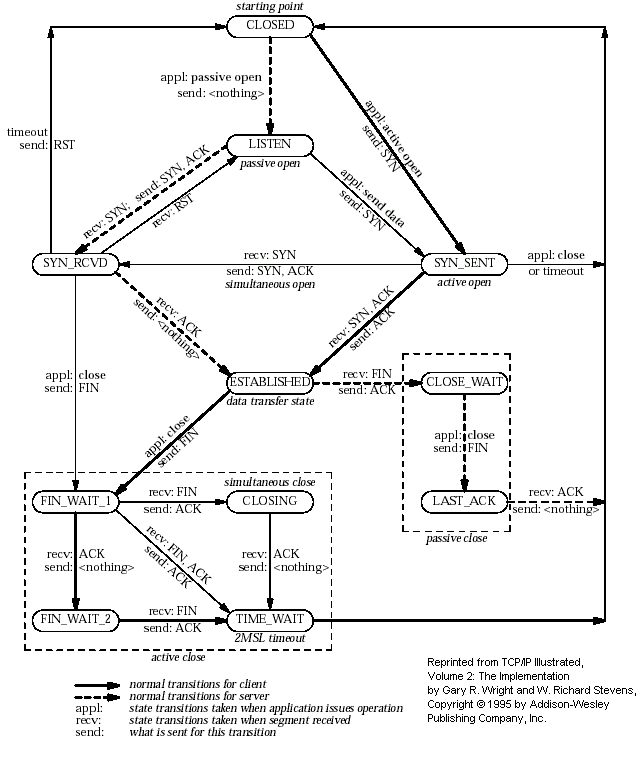
\includegraphics[width=\textwidth]{figures/tcpstate}
\caption{TCP state diagram}
\label{fig:tcp_states}
\end{figure}

\subsection{Flow control}
\label{subsec:flow_control}

The TCP module of the receiver buffers the data of incoming segments.
This buffer has a limited capacity, so it is desirable to notify the sender
about how much data the client can accept. The sender stops the transmission
if this space exhausted.

In TCP every ACK segment holds a Window field; this is the available space
in the receiver buffer. When the sender reads the Window, it can send at most
Window unacknowledged bytes.

\subsubsection*{Window Scale option}

% RFC1323
The TCP segment contains a 16-bit field for the Window, thus allowing at most
65535 byte windows. If the network bandwidth and latency is large, it is surely
too small. The sender should be able to send bandwitdh*latency bytes without
receiving ACKs.

For this purpose the Window Scale (WS) option had been introduced in RFC1323.
This option specifies a scale factor used to interpret the value of the Window field.
The format is the option is:

\begin{center}
\begin{bytefield}{24}
\bitbox{8}{Kind=3} &
\bitbox{8}{Length=3} &
\bitbox{8}{shift.cnt}
\end{bytefield}
\end{center}

If the TCP want to enable window sizes greater than 65535, it should send
a WS option in the SYN segment or SYN/ACK segment (if received a SYN with WS
option). Both sides must send the option in the SYN segment to enable window scaling,
but the scale in one direction might differ from the scale in the other direction.
The $shift.cnt$ field is the 2-base logarithm of the window scale of the sender.
Valid values of $shift.cnt$ are in the $[0,14]$ range.

\subsubsection*{Persistence timer}

When the reciever buffer is full, it sends a 0 length window in the ACK segment
to stop the sender. Later if the application reads the data,
it will repeat the last ACK with an updated window to resume data sending.
If this ACK segment is lost, then the sender is not notified, so a deadlock
happens.

To avoid this situation the sender starts a Persistence Timer when it received
a 0 size window. If the timer expires before the window is increased it send
a probe segment with 1 byte of data. It will receive the current window of the
receiver in the response to this segment.

\subsubsection*{Keepalive timer}

TCP keepalive timer is used to detect dead connections.

\subsection{Transmission policies}
\label{subsec:trans_policies}

\subsubsection*{Retransmissions}

% source: RFC1222 4.3.2.1 and Tannenbaum 6.5.10

When the sender TCP sends a TCP segment it starts a
retransmission timer.
If the ACK arrives before the timer expires it is stopped,
otherwise it triggers a retransmission of the segment.

If the retransmission timeout (RTO) is too high, then lost segments
causes high delays, if it is too low, then the receiver gets
too many useless duplicated segments. For optimal behaviour, the
timeout must be dynamically determined.

Jacobson suggested to measure the RTT mean and deviation
and apply the timeout:

$$ RTO = RTT + 4 * D $$

Here RTT and D are the measured smoothed roundtrip time and its
smoothed mean deviation. They are initialized to 0 and updated each time an
ACK segment received according to the following formulas:

$$ RTT = \alpha*RTT + (1-\alpha) * M $$

$$ D = \alpha*D + (1-\alpha)*|RTT-M| $$

where $M$ is the time between the segments send and the acknowledgment
arrival. Here the $\alpha$ smoothing factor is typically $7/8$.

One problem may occur when computing the round trip: if the
retransmission timer timed out and the segment is sent again,
then it is unclear that the received ACK is a response to the
first transmission or to the second one. To avoid confusing the
RTT calculation, the segments that have been retransmitted
do not update the RTT. This is known as Karn's modification.
He also suggested to double the $RTO$ on each failure until the
segments gets through (``exponential backoff'').

\subsubsection*{Delayed ACK algorithm}

% RFC1122 4.2.3.2

A host that is receiving a stream of TCP data segments can
increase efficiency in both the Internet and the hosts by
sending fewer than one ACK (acknowledgment) segment per data
segment received; this is known as a "delayed ACK" [TCP:5].

Delay is max. 500ms.

A delayed ACK gives the application an opportunity to
update the window and perhaps to send an immediate
response.  In particular, in the case of character-mode
remote login, a delayed ACK can reduce the number of
segments sent by the server by a factor of 3 (ACK,
window update, and echo character all combined in one
segment).

In addition, on some large multi-user hosts, a delayed
ACK can substantially reduce protocol processing
overhead by reducing the total number of packets to be
processed [TCP:5].  However, excessive delays on ACK's
can disturb the round-trip timing and packet "clocking"
algorithms [TCP:7].

% RFC2581 3.2

a TCP receiver SHOULD send an immediate ACK
when the incoming segment fills in all or part of a gap in the
sequence space.

\subsubsection*{Nagle's algorithm}

RFC896 describes the ``small packet problem": when the application
sends single-byte messages to the TCP, and it transmitted immediatly
in a 41 byte TCP/IP packet (20 bytes IP header, 20 bytes TCP header,
1 byte payload), the result is a 4000\% overhead that can cause
congestion in the network.

The solution to this problem is to delay the transmission until
enough data received from the application and send all collected
data in one packet. Nagle proposed that
when a TCP connection has outstanding data that has not
yet been acknowledged, small segments should not be sent
until the outstanding data is acknowledged.

\subsubsection*{Silly window avoidance}

The Silly Window Syndrome (SWS) is described in RFC813. It occurs when
a TCP receiver advertises a small window and the TCP sender immediately
sends data to fill the window. Let's take the example when the sender
process writes a file into the TCP stream in big chunks, while the
receiver process reads the bytes one by one. The first few bytes
are transmitted as whole segments until the receiver buffer
becomes full. Then the application reads one
byte, and a window size 1 is offered to the sender. The sender sends
a segment with 1 byte payload immediately, the receiver buffer becomes
full, and after reading 1 byte, the offered window is 1 byte again.
Thus almost the whole file is transmitted in very small segments.

In order to avoid SWS, both sender and receiver must try to avoid this
situation. The receiver must not advertise small windows and the sender
must not send small segments when only a small window is advertised.

In RFC813 it is offered that
\begin{enumerate}
  \item the receiver should not advertise windows that is smaller than the maximum
        segment size of the connection
  \item the sender should wait until the window is large enough for a maximum sized
        segment.
\end{enumerate}

\subsubsection*{Timestamp option}

Efficient retransmissions depends on precious RTT measurements.
Packet losses can reduce the precision of these measurements radically.
When a segment lost, the ACKs received in that window can not be used;
thus reducing the sample rate to one RTT data per window. This is
unacceptable if the window is large.

The proposed solution to the problem is to use a separate timestamp
field to connect the request and the response on the sender side.
The timestamp is transmitted as a TCP option. The option contains two
32-bit timestamps:

\begin{center}
\begin{bytefield}{80}
\bitbox{8}{Kind=5} &
\bitbox{8}{Length=10} &
\bitbox{32}{TS Value} &
\bitbox{32}{TS Echo Reply} &
\end{bytefield}
\end{center}

Here the TS Value (TSVal) field is the current value of the timestamp
clock of the TCP sending the option, TS Echo Reply (TSecr) field is
0 or echoes the timestamp value of that was sent by the remote TCP.
The TSscr field is valid only in ACK segments that acknowledges new
data. Both parties should send the TS option in their SYN segment
in order to allow the TS option in data segments.

The timestamp option can also be used for PAWS (protection against wrapped
sequence numbers).


\subsection{Congestion control}

Flow control allows the sender to slow down the transmission when the
receiver can not accept them because of memory limitations. However
there are other situations when a slow down is desirable. If the sender
transmits a lot of data into the network it can overload the processing
capacities of the network nodes, so packets are lost in the network
layer.

For this purpose another window is maintained at the sender side, the
congestion window (CWND). The congestion window is a sender-side limit
on the amount of data the sender can transmit into the network before
receiving ACK. More precisely, the sender can send at most max(CWND, WND)
bytes above SND.UNA, therefore $ SND.NXT < SND.UNA + max(CWND, WND) $ is
guaranteed.

The size of the congestion window is dinamically determined by monitoring
the state of the network.

% RFC2581
%
% Definitions:
% SMSS: sender maximum segment size
% RMSS: receiver maximum segment size (default 536)
% rwnd: most recently advertised receiver window
% IW: initial sender's congestion window
% LW: loss window, size of congestion window after a TCP sender detects loss
% RW: restart window, size of congestion window after a TCP restarts transmission after an idle period
% fligth size: amount of data has been sent but not yet acknowledged
% cwnd: congestion window, sender-size limit on the amount of data the sender
%       can transmit into the network before receiving an ACK
% rwnd: receiver advertised window, receiver-side limit on the amount of outstanding data
% sstresh: whether slow start or congestion avoidance used
%
% IW <= 2*MSS


\subsubsection*{Slow Start and Congestion Avoidance}

There are two algorithm that updates the congestion window, ``Slow Start''
and ``Congestion Avoidance''. They are specified in RFC2581.

\begin{pseudocode}
$cwnd \gets 2*SMSS$
$ssthresh \gets $ upper bound of the window (e.g. $65536$)
whenever ACK received
  if $cwnd < ssthresh$
    $cwnd \gets cwnd + SMSS$
  otherwise
    $cwnd \gets cwnd + SMSS*SMSS/cwnd$
whenever packet loss detected
  $cwnd \gets SMSS$
  $ssthresh \gets max(FlightSize/2, 2*SMSS)$
\end{pseudocode}

Slow Start means that when the connection opened the sender initially
sends the data with a low rate. This means that the initial
window (IW) is at most 2 MSS, but no more than 2 segments. If there was no packet loss,
then the congestion window is increased rapidly, it is doubled in each flight.
When a packet loss is detected, the congestion window is reset to 1 MSS (loss window, LW)
and the ``Slow Start'' is applied again.

\begin{note}
RFC3390 increased the IW to roughly 4K bytes: $min(4*MSS, max(2*MSS, 4380))$.
\end{note}

When the congestion window reaches a certain limit (slow start threshold),
the ``Congestion Avoidance'' algorithm is applied. During ``Congestion Avoidance''
the window is incremented by 1 MSS per round-trip-time (RTT). This is usually
implemented by updating the window according to the $ cwnd += SMSS*SMSS/cwnd $
formula on every non-duplicate ACK.

The Slow Start Threshold is updated when a packet loss is detected.
It is set to $max(FlightSize/2, 2*SMSS)$.

How the sender estimates the flight size? The data sent, but not yet acknowledged.

How the sender detect packet loss? Retransmission timer expired.


\subsubsection*{Fast Retransmit and Fast Recovery}

RFC2581 specifies two additional methods to increase the efficiency
of congestion control: ``Fast Retransmit'' and ``Fast Recovery''.

``Fast Retransmit'' requires that the receiver signal the event,
when an out-of-order segment arrives. It is achieved by sending
an immediate duplicate ACK. The receiver also sends an immediate
ACK when the incoming segment fills in a gap or part of a gap.

When the sender receives the duplicated ACK it knows that some
segment after that sequence number is received out-of-order or
that the network duplicated the ACK. If 3 duplicated ACK received
then it is more likely that a segment was dropped or delayed.
In this case the sender starts to retransmit the segments
immediately.

``Fast Recovery'' means that ``Slow Start'' is not applied
when the loss is detected as 3 duplicate ACKs. The arrival
of the duplicate ACKs indicates that the network is not fully
congested, segments after the lost segment arrived, as well
the ACKs.

% Details?
%
%    1.  When the third duplicate ACK is received, set ssthresh to no more
%        than the value given in equation 3.
%
%    2.  Retransmit the lost segment and set cwnd to ssthresh plus 3*SMSS.
%        This artificially "inflates" the congestion window by the number
%        of segments (three) that have left the network and which the
%        receiver has buffered.
%
%    3.  For each additional duplicate ACK received, increment cwnd by
%        SMSS.  This artificially inflates the congestion window in order
%        to reflect the additional segment that has left the network.
%
%    4.  Transmit a segment, if allowed by the new value of cwnd and the
%        receiver's advertised window.
%
%    5.  When the next ACK arrives that acknowledges new data, set cwnd to
%        ssthresh (the value set in step 1).  This is termed "deflating"
%        the window.
%
%        This ACK should be the acknowledgment elicited by the
%        retransmission from step 1, one RTT after the retransmission
%        (though it may arrive sooner in the presence of significant out-
%        of-order delivery of data segments at the receiver).
%        Additionally, this ACK should acknowledge all the intermediate
%        segments sent between the lost segment and the receipt of the
%        third duplicate ACK, if none of these were lost.

\subsubsection*{Loss Recovery Using Limited Transmit}

If there is not enough data to be send after a lost segment,
then the Fast Retransmit algorithm is not activated, but the
costly retranmission timeout used.

RFC3042 suggests that the sender TCP should send a new data segment
in response to each of the first two duplicate acknowledgement. Transmitting
these segments increases the probability that TCP can recover from a single
lost segment using the fast retransmit algorithm, rather than using a costly
retransmission timeout.

\subsubsection*{Selective Acknowledgments}

% RFC2018

With selective
acknowledgments (SACK), the data receiver can inform the sender about all
segments that have arrived successfully, so the sender need
retransmit only the segments that have actually been lost.

With the help of this information the sender can detect
\begin{itemize}
  \item replication by the network
  \item false retransmit due to reordering
  \item retransmit timeout due to ACK loss
  \item early retransmit timeout
\end{itemize}


In the congestion control algorithms described so far
the sender has only rudimentary information about which
segments arrived at the receiver. On the other hand
the algorithms are implemented completely on the sender side,
they only require that the client sends immediate ACKs on
duplicate segments. Therefore they can work in a heterogenous
environment, e.g. a client with Tahoe TCP can communicate with
a NewReno server. On the other hand SACK must be supported by
both endpoint of the connection to be used.

If a TCP supports SACK it includes the \emph{SACK-Permitted} option
in the SYN/SYN-ACK segment when initiating the connection.
The SACK extension enabled for the connection if the \emph{SACK-Permitted}
option was sent and received by both ends. The option occupies
2 octets in the TCP header:

\begin{center}
\begin{bytefield}{16}
\bitbox{8}{Kind=4} &
\bitbox{8}{Length=2}
\end{bytefield}
\end{center}

If the SACK is enabled then the data receiver adds SACK option
to the ACK segments. The SACK option informs the sender about
non-contiguous blocks of data that have been received and queued.
The meaning of the \emph{Acknowledgement Number} is unchanged,
it is still the cumulative sequence number. Octets received
before the \emph{Acknowledgement Number} are kept by the receiver,
and can be deleted from the sender's buffer. However the receiver
is allowed to drop the segments that was only reported in the SACK
option.

The \emph{SACK} option contains the following fields:

\begin{center}
\begin{bytefield}{32}
\bitbox[]{16}{} &
\bitbox{8}{Kind=5} &
\bitbox{8}{Length} \\
\bitbox{32}{Left Edge of 1st Block} \\
\bitbox{32}{Right Edge of 1st Block} \\
\wordbox[]{1}{$\vdots$ \\[1ex]} \\
\bitbox{32}{Left Edge of nth Block} \\
\bitbox{32}{Right Edge of nth Block}
\end{bytefield}
\end{center}

Each block represents received bytes of data that are
contiguous and isolated with one exception: if a segment
received that was already ACKed (i.e. below $RCV.NXT$),
it is included as the first block of the \emph{SACK} option.
The purpose is to inform the sender about a spurious retransmission.

Each block in the option occupies 8 octets. The TCP header
allows 40 bytes for options, so at most 4 blocks can be
reported in the \emph{SACK} option (or 3 if TS option is also used).
The first block is used for reporting the most recently received
data, the following blocks repeats the most recently reported
SACK blocks. This way each segment is reported at least 3 times,
so the sender receives the information even if some ACK segment is
lost.


\textbf{SACK based loss recovery}

% RFC3517: loss recovery based on SACK

Now lets see how the sender can use the information in the
\emph{SACK} option. First notice that it can give a better
estimation of the amount of data outstanding in the network
(called $pipe$ in RFC3517).
If $highACK$ is the highest ACKed sequence number, and
$highData$ of the highest sequence number transmitted,
then the bytes between $highACK$ and $highData$ can be
in the network. However $ pipe \neq highData - highACK $
if there are lost and retransmitted segments:

$$ pipe = highData - highACK - lostBytes + retransmittedBytes $$

A segment is supposed to be lost if it was not received
but 3 segments recevied that comes after this segment in the sequence
number space.
This condition is detected by the sender by receiving
either 3 discontiguous SACKed blocks, or at least
$3*SMSS$ SACKed bytes above the sequence numbers of the
lost segment.

The transmission of data starts with a \emph{Slow Start} phase.
If the loss is detected by 3 duplicate ACK, the sender
goes into the recovery state: it sets
$cwnd$ and $ssthresh$ to $FlightSize / 2$.
It also remembers the $highData$ variable, because
the recovery state is left when this sequence number
is acknowledged.

In the recovery state it sends data
until there is space in the congestion window (i.e. $cwnd-pipe >= 1 SMSS$)
The data of the segment is choosen by the following rules (first rule that applies):

\begin{enumerate}
  \item send segments that is lost and not yet retransmitted
  \item send segments that is not yet transmitted
  \item send segments that is not yet retransmitted and possibly fills a gap
        (there is SACKed data above it)
\end{enumerate}

If there is no data to send, then the sender waits for the next ACK, updates
its variables based on the data of the received ACK, and then try to transmit
according to the above rules.

If an RTO occurs, the sender drops the collected SACK information and
initiates a Slow Start. This is to avoid a deadlock when the receiver
dropped a previously SACKed segment.

% highACK: highest ACKed sequence number
%
% highData: highest sequence number transmitted
%
% highRxt: highest sequence number which has been retransmitted
%
%
% Normal phase: before the first loss, until 3 duplicate ACK
%
% Loss recovery phase: until ACK for RecoveryPoint received
%
% On the transition to loss recovery phase
% \begin{enumerate}
%   \item RecoveryPoint=HighData
%   \item ssthresh=cwnd=FlightSize/2
%   \item compute \emph{pipe}
% \end{enumerate}
%
% In the loss recovery phase, for each incoming ACK:
%
% \begin{enumerate}
%   %\Alph
%   \item if cumulative ACK above RecoveryPoint, leave loss recovery phase
%   \item update SACK info and compute pipe
%   \item if $cwnd-pipe >= 1 SMSS$ send one or more segments (if there is data to send)
%   \item update HighRxt, HighData according to the sent bytes
%   \item increment $pipe$ by the amount of data sent
%   \item if $cwnd-pipe >= 1 SMSS$, continue sending
% \end{enumerate}
%
% Which bytes to be send are determined as follows:
%
% \begin{enumerate}
%   \item if there is a byte which is lost and not yet retransmitted, send that in 1 segment
%   \item otherwise if there is unsent data, send that in 1 segment
%   \item otherwise if there is not yet retransmitted data, and above that there is SACKed data, send that
%   \item otherwise there is no data to send
% \end{enumerate}


\section{TCP module}

The \nedtype{Tcp} simple module is the main implementation of the TCP protocol in the INET framework.
Other implementation are described in section \ref{sec:other_tcp}.
The \nedtype{Tcp} module as other transport protocols work above the network layer and below the application
layer, therefore it has gates to be connected with the IPv4 or IPv6 network (ipIn/ipOut or ipv6In/ipv6Out),
and with the applications (appIn[k], appOut[k]).
One \nedtype{Tcp} module can serve several application modules, and several
connections per application. The $k$th application connects to \nedtype{Tcp}'s
\ttt{appIn[k]} and \ttt{appOut[k]} ports.

The TCP module usually specified by its module interface
(\nedtype{ITcp}) in the NED definition of hosts, so it can be replaced with any implementation
that communicates through the same gates.

\subsection{Statistics}

The \nedtype{Tcp} module collects the following vectors:

\begin{tabular}{l p{10cm}}
  \ttt{send window} & $SND.WND$ \\
  \ttt{receive window} & $RCV.WND$, after SWS avoidance applied \\
  \ttt{advertised window} & $RCV.NXT + RCV.WND$ \\
  \ttt{sent seq} & \emph{Sequence Number} of the sent segment \\
  \ttt{sent ack} & \emph{Acknowledgement Number} of the sent segment \\
  \ttt{rcvd seq} & \emph{Sequence Number} of the received segment \\
  \ttt{rcvd ack} & \emph{Acknowledgement Number} of the received segment \\
  \ttt{unacked bytes} & number of sent and unacknowledged bytes ($max of SND.NXT - SND.UNA$) \\
  \ttt{rcvd dupAcks} & number of duplicate acknowledgements, reset to 0 when $SND.UNA$ advances \\
  \ttt{pipe} & the value of the SACK $pipe$ variable
               (estimated number of bytes outstanding in the network) \\
  \ttt{sent sacks} & number of SACK blocks sent \\
  \ttt{rcvd sacks} & number of SACK blocks received \\
  \ttt{rcvd oooseg} & number of received out-of-order segments \\
  \ttt{rcvd naseg} & number of received unacceptable segments (outside the receive window) \\
  \ttt{rcvd sackedBytes} & total amount of SACKed bytes in the buffer of the sender \\
  \ttt{tcpRcvQueueBytes} & number of bytes in the receiver's buffer \\
  \ttt{tcpRcvQueueDrops} & number of bytes dropped by the receiver (not enough buffer) \\
  \ttt{cwnd} & congestion window \\
  \ttt{ssthresh} & slow start threshold \\
  \ttt{measured RTT} & measured round trip time \\
  \ttt{smoothed RTT} & smoothed round trip time \\
  \ttt{RTTVAR} & measured smoothed variance of round trip time \\
  \ttt{RTO} & retransmission timeout \\
  \ttt{numRTOs} & number of retransmission timeouts occured \\
\end{tabular}

If the \fpar{recordStats} parameter is set to \fkeyword{false}, then none
of these output vectors are generated.

% \subsection{Animation effects}
%
% TCP module text: number of connections sorted by state
%
% log, log verbose

\section{Other TCP implementations}
\label{sec:other_tcp}

INET contains two other implementation of the TCP protocol:
\nedtype{TCP\_lwIP} and \nedtype{TCP\_NSC}.
All TCP modules implements the \nedtype{ITcp} interface and
communicate with the application and the IP layer through the
same interface. Therefore they can be interchanged and can
operate with each other. See \ffilename{examples/inet/tcpclientserver/omnetpp.ini}
how to parametrize \nedtype{StandardHost}s to use the different
implementations.

\subsection{TCP LWIP}

lwIP is a light-weight implementation of the TCP/IP protocol suite
that was originally written by Adam Dunkels of the Swedish Institute of
Computer Science. The current development homepage is
\url{http://savannah.nongnu.org/projects/lwip/}.

The implementation targets embedded devices: it has
very limited resource usage (it works ``with tens of kilobytes of RAM and
around 40 kilobytes of ROM'') and does not require an underlying OS.

The \nedtype{TCP\_lwIP} simple module is based on the 1.3.2 version of
the lwIP sources.

Features:

\begin{compactitem}
\item delayed ACK
\item Nagle's algorithm
\item round trip time estimation
\item adaptive retransmission timeout
\item SWS avoidance
\item slow start threshold
\item fast retransmit
\item fast recovery
\item persist timer
\item keep-alive timer
\end{compactitem}

\subsubsection*{Limitations}

\begin{itemize}
  \item only MSS and TS TCP options are supported. The TS option is turned off
        by default, but can be enabled by defining LWIP\_TCP\_TIMESTAMPS to 1
        in \ffilename{lwipopts.h}.
  \item \fvar{fork} must be \fkeyword{true} in the passive open command
  \item The status request command (TCP\_C\_STATUS) only reports the
          local and remote addresses/ports of the connection and
          the MSS, SND.NXT, SND.WND, SND.WL1, SND.WL2, RCV.NXT, RCV.WND variables.
\end{itemize}

% lwIP license file missing from INET source
% FIXME TCP_lwIP uses only connId to identify the connection instead of (connId,appGateIndex)
% FIXME status command returns message kind TCP_C_STATUS instead of TCP_I_STATUS

\subsubsection*{Statistics}

The \nedtype{TCP\_lwIP} module generates the following vector files:

\begin{itemize}
  \item \ttt{send window}: value of the $SND.WND$ variable
  \item \ttt{sent seq}: \emph{Sequence Number} of the sent segment
  \item \ttt{sent ack}: \emph{Acknowledgment Number } of the sent segment
  \item \ttt{receive window}: value of the $RCV.WND$ variable
  \item \ttt{rcvd seq}: \emph{Sequence Number} of the received segment
  \item \ttt{rcvd acq}: \emph{Acknowledgment Number} of the received segment
\end{itemize}

% FIXME the following vectors are created, but not used (copy paste?):
%       'sent sacks', 'advertised window', 'rcvd sacks', 'unacked bytes',
%       'rcvd dupAcks', 'pipe', 'rcvd oooseg', 'rcvd sackedBytes',
%       'tcpRcvQueueBytes', 'tcpRcvQueueDrops'
The creation of these vectors can be disabled by setting the \fpar{recordStats}
parameter to \fkeyword{false}.


\subsection{TCP NSC}

Network Simulation Cradle (NSC) is a tool that allow real-world TCP/IP network stacks
to be used in simulated networks. The NSC project is created by Sam Jansen
and available on \url{http://research.wand.net.nz/software/nsc.php}. NSC currently
contains Linux, FreeBSD, OpenBSD and lwIP network stacks, altough on 64-bit
systems only Linux implementations can be built.

To use the \nedtype{TCP\_NSC} module you should download the
\ffilename{nsc-0.5.2.tar.bz2} package and follow the instructions
in the \ffilename{<inet\_root>/3rdparty/README} file to build it.

\begin{warning}
Before generating the INET module, check that the \emph{opp\_makemake} call
in the make file (\ffilename{<inet\_root>/Makefile}) includes the
\emph{-DWITH\_TCP\_NSC} argument. Without this option the \nedtype{TCP\_NSC}
module is not built. If you build the INET library from the IDE, it is enough
to enable the \emph{TCP (NSC)} project feature.
\end{warning}

\subsubsection*{Parameters}

The \nedtype{TCP\_NSC} module has the following parameters:

\begin{itemize}
  \item \fpar{stackName}: the name of the TCP implementation to be used.
  Possible values are: \ttt{liblinux2.6.10.so}, \ttt{liblinux2.6.18.so},
  \ttt{liblinux2.6.26.so}, \ttt{libopenbsd3.5.so}, \ttt{libfreebsd5.3.so} and
  \ttt{liblwip.so}. (On the 64 bit systems, the \ttt{liblinux2.6.26.so} and
  \ttt{liblinux2.6.16.so} are available only).

  \item \fpar{stackBufferSize}: the size of the receive and send buffer of
  one connection for selected TCP implementation.
  The NSC sets the \fvar{wmem\_max}, \fvar{rmem\_max}, \fvar{tcp\_rmem}, \fvar{tcp\_wmem}
  parameters to this value on linux TCP implementations. For details, you can see
  the NSC documentation.
\end{itemize}

\subsubsection*{Statistics}

The \nedtype{TCP\_NSC} module collects the following vectors:

\begin{itemize}
  \item \ttt{sent seq} \emph{Sequence Number} of the sent TCP segment
  \item \ttt{sent ack} \emph{Acknowledgment Number} of the sent TCP segment
  \item \ttt{rcvd seq} \emph{Sequence Number} of the received TCP segment
  \item \ttt{rcvd ack} \emph{Acknowledgement Number} of the received TCP segment
\end{itemize}

\subsubsection*{Limitations}

\begin{itemize}
\item Because the kernel code is not reentrant, NSC creates a record containing
the global variables of the stack implementation. By default there is room
for 50 instance in this table, so you can not create more then 50 instance
of \nedtype{TCP\_NSC}. You can increase the \fvar{NUM\_STACKS} constant
in \ffilename{num\_stacks.h} and recompile NSC to overcome this limitation.

\item The \nedtype{TCP\_NSC} module does not supprt TCP\_TRANSFER\_OBJECT
data transfer mode.

\item The MTU of the network stack fixed to 1500, therefore MSS is 1460.

\item TCP\_C\_STATUS command reports only local/remote addresses/ports and
      current window of the connection.

\end{itemize}

% local address: 1.0.0.253, gateway address: 1.0.0.254, remote addresses: 2.0.0.1, 2.0.0.2, ...

% FIXME connections are identified by connId, not by (appGateIndex,connId) as in TCP module.
% FIXME TCP_NSC_Connection::getSocket() and TCP_NSC_Connection::do_checkedclose() are declared but not implemented


%%% Local Variables:
%%% mode: latex
%%% TeX-master: "usman"
%%% End:


\cleardoublepage

\chapter{The SCTP Model}
\label{cha:sctp}


\section{Overview}

Blah blah blah


%%% Local Variables:
%%% mode: latex
%%% TeX-master: "usman"
%%% End:


\cleardoublepage

\chapter{Internet Routing}
\label{cha:routing}

TODO

%%% Local Variables:
%%% mode: latex
%%% TeX-master: "usman"
%%% End:


\cleardoublepage

\ifdraft TODO

\chapter{Differentiated Services}
\label{cha:diffserv}

TODO communication between components

\fi


%%% Local Variables:
%%% mode: latex
%%% TeX-master: "usman"
%%% End:



\cleardoublepage

\chapter{The MPLS Models}
\label{cha:mpls}

TODO how to set up/tear down label switched paths; etc.

\section{MPLS Operation}

The following algorithm is carried out by the MPLS module:

\begin{verbatim}
Step 1: - Check which layer the packet is coming from
Alternative 1: From layer 3
    Step 1: Find and check the next hop of this packet
    Alternative 1: Next hop belongs to this MPLS cloud
        Step 1: Encapsulate the packet in an MPLS packet with
        IP_NATIVE_LABEL label
        Step 2: Send to the next hop
        Step 3: Return
    Alternative 2: Next hop does not belong to this MPLS cloud
        Step 1: Send the packet to the next hop
Alternative 2: From layer 2
    Step 1: Record the packet incoming interface
    Step 2: - Check if the packet is for this LSR
    Alternative 1: Yes
        Step 1: Check if the packet has label
        Alternative 1: Yes
            Step 1: Strip off all labels and send the packet to L3
            Step 2: Return
        Alternative 2: No
            Step 1: Send the packet to L3
            Step 2: Return
    Alternative 2: No
        Step 1: Continue to the next step
    Step 3: Check the packet type
    Alternative 1: The packet is native IP
        Step 1: Check the LSR type
        Alternative 1: The LSR is an Ingress Router
            Step 1: Look up LIB for outgoing label
            Alternative 1: Label cannot be found
                Step 1: Check if the label for this FEC is being requested
                Alternative 1: Yes
                    Step 1: Return
                Alternative 2: No
                    Step 1: Store the packet with FEC id
                    Step 2: Do request the signalling component
                    Step 3: Return
            Alternative 2: Label found
                Step 1: Carry out the label operation on the packet
                Step 2: Forward the packet to the outgoing interface found
                Step 3: Return
        Alternative 2: The LSR is not an Ingress Router
            Step 1: Print out the error
            Step 2: Delete the packet and return
    Alternative 2: The packet is MPLS
        Step 1: Check the LSR type
        Alternative 1: The LSR is an Egress Router
            Step 1: POP the top label
            Step 2: Forward the packet to the outgoing interface found
            Step 3: Return
        Alternative 2: The LSR is not an Egress Router
            Step 1: Look up LIB for outgoing label
            Alternative 1: Label cannot be found
                Step 1: Check if the label for this FEC is being requested
                Alternative 1: Yes
                    Step 1: Return
                Alternative 2: No
                    Step 1: Store the packet with FEC id
                    Step 2: Do request the signalling component
                    Step 3: Return
            Alternative 2: Label found
                Step 1: Carry out the label operation on the packet
                Step 2: Forward the packet to the outgoing interface found
                Step 3: Return
Step 2: Return
\end{verbatim}


\section{LDP Message Processing}

The simulation follows message processing rules specified in RFC 3036
(LDP Specification). A summary of the algorithm used in the RFC is
presented below.

\subsection{Label Request Message processing}

An LSR may transmit a Request message under any of the conditions below:

\begin{itemize}
  \item The LSR recognizes a new FEC via the forwarding tale, and the next hop
    is its LDP peer. The LIB of this LSR does not have a mapping from the
    next hop for the given FEC.
  \item Network topology changes, the next hop to the FEC is no longer valid
    and new mapping is not available.
  \item The LSR receives a Label Request for a FEC from an upstream LDP and it
    does not have label binding information for this FEC. The FEC next hop
    is an LDP peer.
\end{itemize}

Upon receiving a Label Request message, the following procedures will be
performed:

\begin{verbatim}
Step 1: Extract the FEC from the message and locate the incoming interface
        of the message.
Step 2: Check whether the FEC is an outstanding FEC.
    Alternative 1: This FEC is outstanding
        Step 1: Return
    Alternative 2: This FEC is not outstanding
        Step 1: Continue
Step 3: Check if there is an exact match of the FEC in the routing table.
    Alternative 1: There is an exact match
        Step 1: Continue
    Alternative 2: There is no match
        Step 1: Construct a Notification message of No route and
                send this message back to the sender.
Step 4: Make query to local LIB to find out the corresponding label.
    Alternative 1: The label found
        Step 1: Construct a Label Mapping message and send over
                the incoming interface.
    Alternative 2: The label cannot be found for this FEC
        Step 1: Construct a new Label Request message and send
                the message out using L3 routing.
        Step 2: Construct a Notification message indicating that the
                label cannot be found.
\end{verbatim}

\subsection{Label Mapping Message processing}

Upon receiving a Label Mapping message, the following procedures will be
performed:

\begin{verbatim}
Step 1: Extract the FEC and the label from the message.
Step 2: Check whether this is an outstanding FEC
    Alternative 1: This FEC is outstanding
        Step 1: Continue
    Alternative 2: This FEC is not outstanding
        Step 1: Send back the server an Notification of Error message.
Step 3: Install the new label to the local LIB using the extracted label,
        FEC and the message incoming interface.
\end{verbatim}

\section{The CSPF Algorithm}

CSPF stands for Constraint Shortest Path First.
This constraint-based routing is executed online by Ingress Router.
The CSPF calculates an optimum explicit route (ER), based on
specific constraints. CSPF relies on a Traffic Engineering Database (TED)
to do those calculations. The resulting route is then used by RSVP-TE.

The CSPF in particular and any constraint based routing process requires following
inputs:

\begin{itemize}
  \item Attributes of the traffic trunks, e.g., bandwidth, link affinities
  \item Attributes of the links of the network, e.g. bandwidth, delay
  \item Attributes of the LSRs, e.g. types of signaling protocols supported
  \item Other topology state information.
\end{itemize}

There has been no standard for CSPF so far. The implementation of CSPF in
the simulation is based on the concept of "induced graph" introduced in RFC
2702. An induced graph is analogous to a virtual topology in an overlay
model. It is logically mapped onto the physical network through the
selection of LSPs for traffic trunks. CSPF is similar to a normal SPF,
except during link examination, it rejects links without capacity or links
that do not match color constraints or configured policy. The CSPF
algorithm used in the simulation has two phases. In the first phase, all
the links that do not satisfy the constraints of bandwidth are excluded
from the network topology. The link affinity is also examined in this
phase. In the second phase, Dijkstra algorithm is performed.

Dijkstra Algorithm:

\begin{verbatim}
Dijkstra(G, w, s):
   Initialize-single-source(G,s);
   S = empty set;
   Q = V[G];
   While Q is not empty {
       u = Extract-Min(Q);
       S = S union {u};
       for each vertex v in Adj[u] {
           relax(u, v, w);
       }
   }
\end{verbatim}

In which:
\begin{itemize}
  \item G: the graph, represented in some way (e.g. adjacency list)
  \item w: the distance (weight) for each edge (u,v)
  \item s (small s): the starting vertex (source)
  \item S (big S): a set of vertices whose final shortest path from s have already been determined
  \item Q: set of remaining vertices, Q union S = V
\end{itemize}





\cleardoublepage

\chapter{Applications}
\label{cha:apps}


\section{Overview}

This chapter describes application models and traffic generators.

Blah blah blah


%%% Local Variables:
%%% mode: latex
%%% TeX-master: "usman"
%%% End:


\cleardoublepage

\chapter{History}
\label{cha:History}

\section{IPSuite to INET Framework (2000-2006)}

The predecessor of the INET framework was written by Klaus
Wehrle, Jochen Reber, Dirk Holzhausen, Volker Boehm, Verena Kahmann,
Ulrich Kaage and others at the University of Karlsruhe during 2000-2001,
under the name IPSuite.

The MPLS, LDP and RSVP-TE models were built as an add-on to IPSuite
during 2003 by Xuan Thang Nguyen (Xuan.T.Nguyen@uts.edu.au) and other
students at the University of Technology, Sydney under supervision of
Dr Robin Brown. The package consisted of around 10,000 LOCs, and was
published at http://charlie.it.uts.edu.au/~tkaphan/xtn/capstone (now
unavailable).

After a period of IPSuite being unmaintained, Andras Varga took over
the development in July 2003. Through a series of snapshot releases in
2003-2004, modules got completely reorganized, documented, and many of them
rewritten from scratch. The MPLS models (including RSVP-TE, LDP, etc)
also got refactored and merged into the codebase.

During 2004, Andras added a new, modular and extensible TCP implementation,
application models, Ethernet implementation and an all-in-one IP model
to replace the earlier, modularized one.

The package was renamed INET Framework in October 2004.

Support for wireless and mobile networks got added during summer 2005
by using code from the Mobility Framework.

The MPLS models (including LDP and RSVP-TE) got revised and mostly
rewritten from scratch by Vojta Janota in the first half of 2005
for his diploma thesis. After further refinements by Vojta, the new code
got merged into the INET CVS in fall 2005, and got eventually released
in the March 2006 INET snapshot.

The OSPFv2 model was created by Andras Babos during 2004 for his diploma
thesis which was submitted early 2005. This work was sponsored by Andras Varga,
using revenues from commercial OMNEST licenses. After several refinements and fixes,
the code got merged into the INET Framework in 2005, and became part of the
March 2006 INET snapshot.

The Quagga routing daemon was ported into the INET Framework also by Vojta
Janota. This work was also sponsored by Andras Varga. During fall 2005 and
the months after, ripd and ospfd were ported, and the methodology of porting
was refined. Further Quagga daemons still remain to be ported.

Based on experience from the IPv6Suite (from Ahmet Sekercioglu's group at
CTIE, Monash University, Melbourne) and IPv6SuiteWithINET (Andras's effort
to refactor IPv6Suite and merge it with INET early 2005), Wei Yang Ng
(Monash Uni) implemented a new IPv6 model from scratch for the
INET Framework in 2005 for his diploma thesis, under guidance from Andras
who was visiting Monash between February and June 2005. This IPv6 model
got first included in the July 2005 INET snapshot, and gradually refined
afterwards.

The SCTP implementation was contributed by Michael Tuexen, Irene Ruengeler
and Thomas Dreibholz

Support for Sam Jensen's Network Simulation Cradle,
which makes real-world TCP stacks available in simulations was added
by Zoltan Bojthe in 2010.

TCP SACK and New Reno implementation was contributed by Thomas Reschka.

Several other people have contributed to the INET Framework by providing
feedback, reporting bugs, suggesting features and contributing patches;
I'd like to acknowledge their help here as well.



%%% Local Variables:
%%% mode: latex
%%% TeX-master: "usman"
%%% End:


\cleardoublepage

\bibliographystyle{alpha}
\bibliography{inet-manual}


%% no need for the following since 'tocbibind' package
%% \phantomsection
%% \addcontentsline{toc}{chapter}{\indexname}
\printindex

\end{document}

%%% Local Variables:
%%% mode: latex
%%% TeX-master: t
%%% End:
